\documentclass[12pt, a4paper, oneside]{extarticle}
\usepackage[top=3cm, right=2.5cm, bottom=2.5cm, left=3cm]{geometry}
%Support for Greek Language in main body and in math equations
\usepackage[utf8]{inputenc}
\usepackage[english, greek]{babel}

\usepackage{kerkis}

\usepackage[none]{hyphenat}

\usepackage{alphabeta}
\usepackage[LGR, T1]{fontenc}
\usepackage{indentfirst}
\usepackage{xspace}
\usepackage{amsfonts, amsmath, amssymb}
\usepackage{bm}
\numberwithin{equation}{subsection}
\usepackage[none]{hyphenat} %Stops breaking up words (mostly in tables)
\usepackage{fancyhdr}
\usepackage{fancyvrb}
\RecustomVerbatimEnvironment{Verbatim}{Verbatim}{numbers=left,xleftmargin=5mm, commandchars=\\\{\}, frame=single}
\usepackage{color}
\usepackage{listings}
\usepackage{gensymb}
\usepackage{enumitem}
\usepackage{url}
\usepackage[hidelinks]{hyperref}
\usepackage{csquotes}
\usepackage{multirow}
\usepackage{rotating}
\usepackage{pdflscape}
\renewcommand{\lstlistingname}{Κώδικας}

\definecolor{codegreen}{rgb}{0,0.6,0}
\definecolor{codegray}{rgb}{0.5,0.5,0.5}
\definecolor{codepurple}{rgb}{0.58,0,0.82}
\definecolor{backcolour}{rgb}{0.9,0.9,0.9}
 
\lstdefinestyle{nonums}{
    % backgroundcolor=\color{backcolour},   
    commentstyle=\color{codegreen},
    keywordstyle=\bfseries\color{magenta},
    numberstyle=\small\color{codegray},
    stringstyle=\color{codepurple},
    basicstyle=\ttfamily\small,
    breakatwhitespace=false,         
    breaklines=true,                 
    captionpos=b,                    
    keepspaces=true,                 
    % numbers=left,                    
    numbersep=5pt,                  
    showspaces=false,                
    showstringspaces=false,
    showtabs=false,                  
    tabsize=2
}

\lstdefinestyle{withnums}{
    % backgroundcolor=\color{backcolour},   
    commentstyle=\color{codegreen},
    keywordstyle=\bfseries\color{magenta},
    numberstyle=\small\color{codegray},
    stringstyle=\color{codepurple},
    basicstyle=\ttfamily\small,
    breakatwhitespace=false,         
    breaklines=true,                 
    captionpos=b,                    
    keepspaces=true,                 
    numbers=left,                    
    numbersep=5pt,                  
    showspaces=false,                
    showstringspaces=false,
    showtabs=false,                  
    tabsize=2
}

% Create a custom List-Of-Listings
\addto\captionsgreek{%
  \renewcommand{\lstlistlistingname}{Κατάλογος Αλγορίθμων}%
}
% % % % % % % % % % % % % % % % % %


%references preamble
\usepackage{natbib}
\bibliographystyle{agsm}
\def\lat#1{\textlatin{#1}}
\def\cor{\textlatin{Coriolis\ }}
\def\ros{\textlatin{Rossby\ }}


%%%%% EDIT THESE %%%%%%
\newcommand{\theauthor}{Νικόλαος Ανδρεάκος\xspace}
\newcommand{\thetitle}{Μοντελοποίηση παλιρροιϊκής κυκλοφορίας και σχετικών αλγορίθμων\xspace}
\newcommand{\thedate}{Πάτρα, 2019\xspace}

\newcommand{\tmima}{Τμήμα πολιτικών Μηχανικών\xspace}
\newcommand{\proff}{Γεώργιος Μ. Χορς\xspace}
\newcommand{\proffrole}{Αναπληρωτής Καθηγητής\xspace}
%%%%%%%%%%%%%%%%%%%%%%%%%


%Graphics preamble
\usepackage{graphicx, subfigure}  % Allows you to import images.
\usepackage{float} %Allows for control of float positions.
\graphicspath{ {images/} } %folder where images are saved (relative to path)

\usepackage[nottoc, notlot, notlof]{tocbibind}

\linespread{1.5} % Line spacing

\usepackage{lipsum} % for dummy text only
\newenvironment{ComputerFont}{\fontfamily{cmr}\selectfont}{\par}

\pagestyle{fancy}
\fancyhead{}
\fancyfoot{}
\fancyhead[R]{\thetitle}
% \fancyhead[C]{\rightmark}
% \fancyfoot[L]{\rightmark}
\fancyfoot[R]{\thepage}
\renewcommand{\headrulewidth}{1pt}

\newenvironment{ComputerModern}{\fontfamily{<cmr>}\selectfont}{\par}

%page style used for preface, abstract, lists, contents
\fancypagestyle{pagenum}{
	\fancyhead{}
	\fancyfoot{}
	\fancyfoot[R]{\thepage}
	\renewcommand{\headrulewidth}{0pt}
}

\fancypagestyle{appendix}{
	\fancyhead{}
	\fancyfoot{}
	\fancyhead[C]{ΠΑΡΑΡΤΗΜΑ}
	\fancyfoot[R]{\thepage}
	\renewcommand{\headrulewidth}{1pt}
}


\usepackage{titling}

\begin{document}
	\sloppy
	\begin{ComputerFont}
		\begin{titlepage}
			\begin{center}
				
\includegraphics[scale=0.4]{logo_pp}\\
				\Large{\MakeUppercase{\textbf{Πανεπιστήμιο Πατρών}}}\\
				\Large{\textbf{\tmima}}\\
				\vfill
				\line(1,0){400}\\[1mm]
				\LARGE{{\textbf{\thetitle}}}\\[3mm]
				\Large{\MakeUppercase{{Διπλωματική Εργασία}}}\\[1mm]
				\line(1,0){400}\\
				\vfill
				\textbf{\Large{\theauthor}}\\[2mm]
				Επιβλέπων Καθηγητής:\\
				\proff, \proffrole \\
				\vfill
				\thedate \\
			\end{center}
		\end{titlepage}
	\end{ComputerFont}

	\pagenumbering{roman}
	\section*{Πρόλογος}
		\thispagestyle{pagenum}
		\addcontentsline{toc}{section}{\numberline{}Πρόλογος}
		Η παρούσα διπλωματική εργασία εκπονήθηκε στα πλαίσια του προπτυχιακού προγράμματος Πολιτικών Μηχανικών, του Πανεπιστημίου Πατρών. Κύριος στόχος της εργασίας είναι η μοντελοποιήση της κυκλοφορίας σε έναν εξιδανικευμένο κόλπο, με κύρια διέγερση ένα παλιρροϊκό κύμα. Ακόμα, αναφέρονται και κάποια άλλα στοιχεία πολύ χρήσιμα για την επιστήμη του υδραυλικού πολιτικού μηχανικού, η φαινόμενη δύναμη \lat{Coriolis} και το σύστημα \lat{Lorenz}.

		Κύριος, προσωπικός, στόχος μου ήταν η ανάπτυξη λογισμικού, με σύγχρονες προδιαγραφές, όπου να μπορεί να επιλύσει τα φαινόμενα που περιγράφονται στη διπλωματική εργασία επαρκώς, αλλά και ταχέως.

		Εκτός από τις γνώσεις που έλαβα κατά τη διάρκεια υλοποίησης του λογισμικού και της συγγραφής της παρούσας διπλωματικής, το υλικό που παρουσιάζεται είναι ιδιαίτερα χρήσιμο σε κάποιον που ξεκινά να μελετά φαινόμενα κυκλοφορίας.

		Σε αυτό το σημείο, θα ήθελα να ευχαριστήσω θερμά τον κ. Γεώργιο Χορς, Αναπληρωτή Καθηγητή, για την επιστημονική καθοδήγησή του, καθώς και την πολύτιμη βοήθεια που μου προσέφερε κατα τη διάρκεια εκπόνησης αυτής της εργασίας. Η παρουσία του κρίθηκε απαραίτητη στα τελευταία χρόνια των σπουδών μου. Ακόμα, είναι απαραίτητο να αναφερθώ και να ευχαριστήσω την οικογένειά μου και τους φίλους μου στάθηκαν δίπλα μου και με υποστήριξαν στο έργο μου.
		\vspace{20mm}
		\begin{flushright}
			Πάτρα, 2019
		\end{flushright}

		\cleardoublepage

	\section*{Περίληψη}
		\thispagestyle{pagenum}
		\addcontentsline{toc}{section}{\numberline{}Περίληψη}
		Η παρούσα διπλωματική εργασία διαρθρώνεται σε τρία κύρια μέρη.

		Το πρώτο μέρος παρουσιάζεται το σύστημα \lat{Lorenz}. Αναφέρεται ο τρόπος που ανακαλύφθηκε, η χρήση του στο φυσικό κόσμο, καθώς και προτείνεται μία αριθμητική επίλυσή του. Ακόμα, παρουσιάζεται ένα πρόγραμμα με γραφικό περιβάλλον, που αναπτύχθηκε για τα πλαίσια αυτής της διπλωματικής εργασίας, όπου επιλύεται το σύστημα για διάφορες αρχικές συνθήκες που ορίζει ο χρήστης και εμφανίζει ένα κινούμενο γραφικό αποτέλεσμα.

		Στο δεύτερο κεφάλαιο γίνεται αναφορά στη δύναμη \cor και πώς επηρεάζει φαινόμενα που εξελίσσονται στη γη. Γίνεται ανάλυση των ιδιοτήτων αυτής της δύναμης και περιγράφεται το αποτέλεσμά της σε μία κίνηση σε περιστρεφόμενο σύστημα αναφοράς. Επίσης, γίνεται αναφορά και σε φαινόμενα που συνήθως η δύναμη \cor αποτελεί καθοριστικό παράγοντα, όπως για παράδειγμα τα αδρανειακά κύματα. Τέλος, παρουσιάζεται ένα λογισμικό, που επίσης αναπτύχθηκε στα πλαίσια αυτής της διπλωματικής εργασίας, όπου ο χρήστης μπορεί να ορίσει τις αρχικές συνθήκες και να λάβει μία γραφική απεικόνιση της τροχιάς που θα ακολουθήσει ένα σωματίδιο. Το λογισμικό επιστρέφει, ακόμα, κάποιες χρήσιμες παραμέτρους, όπως ο αριθμός \lat{Rossby}.

		Στο τρίτο και τελευταίο κεφάλαιο μοντελοποιείται η κυκλοφορία σε ένα κόλπο, εξιδανικευμένων διαστάσεων, που διεγείρεται από ένα ημιτονοειδές κύμα, που προσομοιάζει ένα αντίστοιχο παλιρροϊκό κύμα. Γίνεται εκτενής ανάλυση και περιγραφή των εξισώσεων που διέπουν ένα τέτοιο πρόβλημα, καθώς και προτείνεται η αριθμητική του λύση μέσω των πεπερασμένων διαφορών. Τέλος, παρουσιάζονται και αναλύονται τα αποτελέσματα διαφόρων επιλύσεων, σε δύο μεγέθη πλεγμάτων και για διαφορετικό χρόνο εκτέλεσης της επίλυσης.
	\cleardoublepage

	% PERIEXOMENA %
	\tableofcontents
		\thispagestyle{pagenum}
		\addcontentsline{toc}{section}{\numberline{}Περιεχόμενα}
	\clearpage

	%katalogos sximatwn
	\addcontentsline{toc}{section}{\numberline{}Κατάλογος Σχημάτων}
		\listoffigures
		\thispagestyle{pagenum}
	\cleardoublepage

	%Katalogos pinawkn
	\addcontentsline{toc}{section}{\numberline{}Κατάλογος Πινάκων}
		\listoftables
		\thispagestyle{pagenum}
	\cleardoublepage

	\addcontentsline{toc}{section}{\numberline{}Κατάλογος Αλγορίθμων}
		% \selectlanguage{english}
		\lstlistoflistings
		\thispagestyle{pagenum}
		% \selectlanguage{greek}
	\cleardoublepage

	%% MAIN  BODY %%
	%%  CORIOLIS  %%
	\pagenumbering{arabic}
	\section{Οπτικό μοντέλο του συστήματος \lat{Lorenz}}
		\subsection{Το σύστημα \lat{Lorenz}}
Tο συστημα \lat{Lorenz}, που μελετήθηκε για πρώτη φορά από τον \lat{Edward Lorenz} στο έργο του \textit{\lat{Deterministic nonperiodic flow}}, \lat{\cite{LOR}}, είναι ένα σύστημα που αποτελείται από συνήθεις διαφορικές εξισώσεις και αποτελεί ένα αξιοσημείωτο παράδειγμα χαοτικού προβλήματος.

Για συγκεκρίμενες τιμές των παραμέτρων, το σύστημα συμπεριφέρεται χαοτικά. Μικρές μεταβολές στις αρχικές συνθήκες καταλήγουν σε τελείως διαφορετική λύση του προβλήματος, που παραμένει ωστόσο ντετερμινιστικό.

Ο ελκυστήρας του \lat{Lorenz}, όπως είναι γνωστό το σύστημα, αποτελεί μία απλοποιημένη μορφή ενός συστήματος εξισώσεων που περιγράφουν την διδιάστατη ροή ενός ρευστού, με ομοίομορφο πάχος $H$ και διαφορά θερμοκρασίας $ΔΤ$, υπό την επήρεια της βαρυτικής επιτάχυνσης $g$, με άνωση $α$, συντελεστή θερμικής μετάδοσης $κ$ και κινηματικό ιξώδες $ν$, \lat{\cite{TABOR}}
\begin{align}
    \dfrac{\partial}{\partial{t}}\left(\nabla^{2} φ\right) &= \dfrac{\partial ψ}{\partial z} \dfrac{\partial}{\partial x}\left(\nabla^{2} ψ\right) - \dfrac{\partial ψ}{\partial x} \dfrac{\partial}{\partial z}\left(\nabla^{2} ψ\right) + ν\nabla^{2}\left(\nabla^{2}ψ\right) + gα\dfrac{dT}{dx} \\
    \dfrac{\partial T}{\partial t} &= \dfrac{\partial{T}}{\partial{z}}\dfrac{\partial{ψ}}{\partial{x}} - \dfrac{\partial{θ}}{\partial{x}}\dfrac{\partial{ψ}}{\partial{z}} + κ\nabla^{2}T + \dfrac{ΔT}{H}\dfrac{\partial{ψ}}{\partial{x}}
\end{align}

όπου $ψ$ η ροϊκή συνάρτηση τέτοια ώστε το διάνυσμα της ταχύτητα $\textbf{u}=\left(u, w\right)$ είναι
\begin{align}
    u &= \dfrac{\partial{ψ}}{\partial{z}} \\
    w &= -\dfrac{\partial{ψ}}{\partial{x}}
\end{align}

Ο \lat{Lorenz} ανακάλυψε τυχαία ότι σε ένα απλοποιημένο σύστημα, του οποίου η λύση είναι συγκεκριμένης μορφής, παρουσιαζεται χαοτική συμπεριφορά
\begin{equation}
    \begin{cases}
        \dfrac{dx}{dt} &= σ\left(y - x\right) \\
        \dfrac{dy}{dt} &= x\left(ρ - z\right) - y \\
        \dfrac{dz}{dt} &= xy - βz 
    \end{cases}
\end{equation}

Το απλοποιημένου του σύστημα συσχετίζει τις ιδιότητες ενός διδιάστατου ρευστου στρώματος, όπου το $x$ είναι ανάλογο του ρυθμού μετάδοσης, το $y$ είναι ανάλογο της διαφοράς θερμοκρασίας κατά μήκος και το $z$ είναι ανάλογο της κατακόρυφης κατανομής της θερμοκρασίας.

Ακόμα εισήγαγε τις θετικές παραμέτρους $σ$, $ρ$ που είναι ανάλογες του αριθμού \lat{Prandtl} και του αριθμού \lat{Rayleigh}, καθώς και το $β$ που είναι χαρακτηριστικό για των φυσικών διαστάσεων του ρευστού στρώματος.

Στο σύστημα εμφανίζονται τρία κρίσιμα σημεία. Το πρώτο $\left(0, 0, 0\right)$ που αντιστοιχεί σε μηδενική μετάδοση και τα 
\begin{align}
    \left( \sqrt{β\left(ρ-1\right)} , \sqrt{β\left(ρ-1\right)} , ρ-1\right) \\
    \left( -\sqrt{β\left(ρ-1\right)} , -\sqrt{β\left(ρ-1\right)} , ρ-1\right)
\end{align}
που αντιστοιχούν σε σταθερή μετάδοση θερμότητας. Το ζεύγος των σημείων είναι ευσταθές μόνο αν 
\begin{equation}
    ρ < σ\dfrac{σ+β+3}{σ-β-1} \Rightarrow σ>β+1
\end{equation}

Οι τιμές που ο \lat{Lorenz} επέλεξε για τις παραμέτρους, για τις οποίες παρουσιάζεται χαοτική συμπεριφορά, είναι
\begin{align}
    σ &= 10 \\
    β &= 8/3 \\
    ρ &= 23
\end{align}

Το σύστημα είναι δύσκολο να αναλυθεί και συνήθως είναι πιο εύκολη η οπτικοποιήση του, μέσω της λύσης του με κάποια υπολογιστική τεχνική. Το οπτικό αποτέλεσμα εμφανίζει τη μορφή μια πεταλούδας ή του αριθμού 8 και αυτός είναι ο λόγος που πήρε το όνομά του το \textit{φαίνομενο της πεταλούδας}, όρο τον οποίο χρησιμοποίησε για πρώτη φορά ο \lat{Edward Lorenz}.

\subsection{Υπολογιστική Επίλυση}

Το σύστημα των διαφορικών εξισώσεων μπορεί να λυθεί εύκολα κάνοντας χρήση μίας υπολογιστικής μεθόδου. Για την παρούσα εργασία επιλέχθηκε η επίλυση μέσω της μεθόδου \textit{\lat{LSODA}}, κυρίως λόγω της της ευκολίας στην υλοποίηση, αλλά και της δυνατότητας του αλγορίθμου να προσαρμόζεται στο σύστημα και να προσαρμόζει και το βήμα ολοκλήρωσης (\lat{\textit{variable step size intergration}}).

Για την υπολογιστική επίλυση χρησιμοποιήθηκε η γλώσσα \textit{\lat{Python}} και το πακέτο αριθμητικής ολοκλήρωσης διαφορικών εξισώσεων \textit{\lat{scipy.intergrate.odeint}}, που χρησιμοποιεί τη βιβλιοθήκη της \textit{\lat{LSODA}} που προέρχεται από τη \textit{\lat{FORTRAN}}. Στο \lat{documentation} της βιβλιοθήκης αριθμητικής ολοκλήρωσης διαφορικών εξισώσεων \textit{\lat{scipy.intergrate.odeint}} περιγράφεται ότι
\begin{displayquote}
    \selectlanguage{english}
    \textit{Solve a system of ordinary differential equations using lsoda from the FORTRAN library odepack.}  \\
    \textit{Solves the initial value problem for stiff or non-stiff systems of first order ode-s:}
    \begin{verbatim}
        dy/dt = func(y, t, ...)  [or func(t, y, ...)]
    \end{verbatim}
    \textit{where y can be a vector.}
\end{displayquote}

Αντίστοιχα το \lat{documentation} της \lat{LSODA} αναφέρει ότι
\begin{displayquote}
    \selectlanguage{english}
    \textit{\textbf{LSODA}, written jointly with L. R. Petzold, solves systems dy/dt = f with a dense or banded Jacobian when the problem is stiff, but it automatically selects between nonstiff (Adams) and stiff (BDF) methods. It uses the nonstiff method initially, and dynamically monitors data in order to decide which method to use.}
\end{displayquote}

\subsection{Αλγόριθμος επίλυσης}
\selectlanguage{english}
\lstset{style=nonums}
\lstinputlisting[nolol=true, language=Python, caption=Lorenz System Solver]{lorenz.py}

\subsection{Γραφικό Περιβάλλον}
	\cleardoublepage
	\section{Δύναμη \lat{Coriolis}}
		Για την κίνηση των σωμάτων θεμελιώθηκαν οι κινηματικοί νόμοι από το Νεύτωνα με το έργο του \textlatin{Principia} (\lat{Philosophiæ Naturalis Principia Mathematica}, 1687). Η νευτώνια κινηματική περιγράφει την κίνηση των αντικειμένων σε ένα αδρανειακό, μη κινούμενο δηλαδή, σύστημα αναφοράς. Όταν εξετάζονται κινήσεις μεγάλης κλίμακας, τέτοιας ώστε η περιστροφή της γης γύρω από τον άξονά της να τις επηρεάζει, η νευτώνια κινηματική δεν μπορεί να τις περιγράψει πλήρως.

Στις εξισώσεις κίνησης ενός σώματος, το οποίο κινείται σε σχέση με ένα περιστρεφόμενο σύστημα αναφοράς, σαν αυτό της περιστρεφόμενης γης, εμφανίζεται μία φαινόμενη δύναμη, η δύναμη \cor. Η δύναμη αυτή πήρε το όνομά της από το Γάλλο επιστήμονα  Γκασπάρ - Γκoυστάβ ντε Κοριόλις (γαλλ. \lat{Gaspard-Gustave de Coriolis}).

Η επιρροή του περιστρεφόμενου συστήματος στην κίνηση του σώματος μπορεί να προσδιοριστεί υπολογίζοντας τον αριθμό \textit{\ros}
\begin{equation}
	Ro = \frac{U}{{Lf}}
\end{equation}
όπου $U$ και $L$ είναι η χαρακτηριστική ταχύτητα και το χαρακτηριστικό μήκος αντίστοιχα, ενώ $f$ η παράμετρος \cor . Ο αριθμός \cor  είναι στην ουσία ο λόγος των αδρανειακών δυνάμεων προς τις δυνάμεις \cor  και είναι χαρακτηριστικός για το σύστημα. Οι δυνάμεις \cor  είναι εμφανείς και ισχυρές και υπερισχύουν των αδρανειακών δυνάμεων, όταν ο αριθμός \ros είναι μικρός. Το σύστημα επέρχεται σε ισορροπία με τη δράση της δύναμης \cor  και της βαθμίδας πίεσης. Η ισορροπία αυτή ονομάζεται \textit{γεωστροφική ισορροπία}. Αντίθετα, όταν ο αριθμός \ros είναι μεγάλος, οι αδρανειακές δυνάμεις υπερισχύουν και το σύστημα έρχεται σε ισορροπία υπό την επίδραση της κεντρομόλου και της φυγόκεντρου δύναμης, όπως ονομάζεται \textit{κυκλοστροφική ισορροπία} (Χαλδούπης, 2015).

\subsection{Παράμετρος \cor \lat{f}}	
Η παράμετρος \cor, γνωστή και ως συχνότητα \cor, εξαρτάται από την ταχύτητα περιστροφής της γης $Ω$ και το γεωγραφικό πλάτος $φ$ εξέλιξης του φαινομένου. Η καμπυλότητα της επιφάνειας της γης μπορεί να αγνοηθεί για αποστάσεις μικρότερες των 100 \lat{km}. Έτσι, τοποθετώντας το σύστημα συντεταγμένων στην επιφάνεια της θάλασσας, με τον άξονα $z$ κατακόρυφα σε αυτή, η παράμετρος \cor \lat{f} μπορεί να θεωρηθεί σταθερή. Η τιμή της παραμέτρου υπολογίζεται ως
\begin{equation}
	f=2Ωsinφ
\end{equation}
Η τιμή αλλάζει πρόσημο κατά τη μετάβαση από το βόρειο προς το νότιο ημισφαίριο, και αντίθετα, ενώ γίνεται 0 στον ισημερινό.

Το όνομα συχνότητα \cor προήλθε από τις αδρανειακές ταλαντώσεις, που έχουν συχνότητα ίση με την παράμετρο \cor. Οι ταλαντώσεις αυτές ονομάζονται και αδρανειακά κύματα. Τα κύματα αυτά είναι εγκάρσια και παρατηρούνται τόσο στην ατμόσφαιρα (πχ. \textit{γεωστροφικός άνεμος}), όσο και στους ωκεανούς και στις λίμνες (\textit{γεωστροφικά ρεύματα}). Τα κύματα τα οποία επηρεάζονται από την κλίση του πυθμένα ονομάζονται κύματα \ros.

\subsection{Μετασχηματισμός θέσης σε περιστρεφόμενο σύστημα αναφοράς}
Θεωρώντας ένα σωματίδιο ακίνητο σε καρτεσιανό αδρανειακό σύστημα αναφοράς, η θέση του περιγράφεται από το διάνυσμα $\bm{X}=e_1x_1+e_2x_2+e_3x_3$. Σε μητρωική μορφή, το διάνυσμα θέσης στο αδρανειακό σύστημα είναι
\begin{equation}
\bm{X}=
\begin{pmatrix}
	e_1 & e_2 & e_3
\end{pmatrix}
\begin{pmatrix}
  x_{1} \\
  x_{2} \\
  x_{3} \\
\end{pmatrix}
\end{equation}

Σε ένα άλλο καρτεσιανό σύστημα, το οποίο έχει περιστραφεί \textit{αριστερόστροφα} σε σχέση με το προηγούμενο κατά μία γωνία $θ$, η θέση του σωματιδίου περιγράφεται από το διάνυσμα 
\begin{equation}
 \label{eq:Xprime}
 \bm{X^{\prime}} =
 \begin{pmatrix}
  x_{1}^{\prime} \\
  x_{2}^{\prime} \\
  x_{3}^{\prime} \\
 \end{pmatrix} = 
 \begin{pmatrix}
  x_{1}cos{θ}+x_{2}sin{θ} \\
  -x_{1}sin{θ}+x_{2}cos{θ} \\
  x_{3} \\
 \end{pmatrix}
\end{equation}
Παρατηρώντας την (\ref{eq:Xprime}), μπορεί να εκλεχθεί ένα μητρώο μετασχηματισμού $\mathbb{R}$ και η θέση του σωματιδίου να περιγράφεται από το διάνυσμα $\bm{X^{\prime}}=\mathbb{E}\mathbb{R}\mathbb{X}$. Το μητρώο αυτό είναι
\begin{equation}
 \label{eq:Rvector}
 \mathbb{R} =
 \begin{pmatrix}
  cos{θ} & sin{θ} & 0 \\
  sin{θ} & cos{θ} & 0 \\
  0      &   0    & 1 \\
 \end{pmatrix}
\end{equation}

\subsection{Περιγραφή του αλγορίθμου}
Η διαδικασία του μετασχηματισμού της θέσης ενός σωματιδίου, που περιγράφηκε παραπάνω, είναι εύκολο να γίνει αλγοριθμικά. Πρέπει να σημειωθεί ότι η διαδικασία αυτή μπορεί να περιγράψει κάθε είδους κίνηση επί του αδρανειακού επιπέδου, καθώς το μόνο απαραίτητο στοιχείο είναι οι καρτεσιανές συντεταγμένες της θέσης του σωματιδίου, οποιαδήποτε στιγμή. Στην κατάστρωση του αλγορίθμου επιλέχθηκε το σώμα να βάλλεται με μία αρχική ταχύτητα $(u, v)$, αντίστοιχα σε κάθε άξονα και έπειτα να ακολουθεί την ευθύγραμμη ομαλή κίνηση. Ακόμα επιλέχθηκε το περιστρεφόμενο σύστημα να περιστρέφεται με σταθερή γωνιακή ταχύτητα, παρόλο που η διαδικασία μπορεί να εφαρμοστεί σε κάθε περίπτωση. Ο λόγος που έγιναν αυτές οι παραδοχές είναι ώστε ο αλγόριθμος να περιγράφει και να αναλύει την κίνηση ενός σωματιδίου στο επίπεδο της γης, καθώς αυτή περιστρέφεται γύρω από τον άξονα της.

'Οπως είναι γνωστό από τη φυσική η θέση ενός σωματιδίου κάθε χρονική στιγμή $i$ δίνεται αναδρομικά από την προηγούμενη
\begin{align}
x_{i} &= x_{i-1}+u\Delta t \\
y_{i} &= y_{i-1}+v\Delta t
\end{align}
όπου $Δt$ είναι ένα απειροστό διάστημα χρόνου και $(u, v)$ οι ταχύτητες σε κάθε άξονα.

Έτσι γνωρίζοντας τη θέση του σωματιδίου στο αδρανειακό σύστημα και ακολουθώντας το μετασχηματισμό (\ref{eq:Xprime}) γίνεται ο υπολογισμός της θέσης του στο περιστρεφόμενο σύστημα. O αλγορίθμου, ο οποίος επιστρέφει τις συντεταγμένες κάθε σημείου της τροχιάς που εκτελεί το σωματίδιο, όπως αυτή αποτυπώνεται στο περιστρεφόμενο σύστημα αναφοράς φαίνεται παρακάτω (βλ. Πίνακα \ref{tab:algCoriolis}).
\begin{table}[h]
	\caption{Αλγόριθμος τροχιάς σημείου σε περιστρεφόμενο σύστημα αναφοράς.}
	\label{tab:algCoriolis}
	\selectlanguage{english}
	\begin{Verbatim}
	\textcolor{green}{ΑΡΧΗ}
	    x0 \textcolor{blue}{=} αρχική θέση στον άξονα x
	    y0 \textcolor{blue}{=} αρχική θέση στον άξονα y
	    θ  \textcolor{blue}{=} 0
	    \textcolor{red}{Για} t \textcolor{blue}{=} 1 \textcolor{red}{έως} t \textcolor{blue}{=} t_Τελικό \textcolor{red}{με_βήμα =} Δt:
	        θ \textcolor{blue}{=} θ \textcolor{blue}{+} Ω \textcolor{blue}{*} Δt
	        x1 \textcolor{blue}{=} x0 \textcolor{blue}{+} u*Δt
	        y1 \textcolor{blue}{=} y0 \textcolor{blue}{+} v*Δt
	        xprime1 \textcolor{blue}{=}  x1*cos(θ) \textcolor{blue}{+} y1*sin(θ)
	        yprime1 \textcolor{blue}{=} \textcolor{blue}{-}x1*sin(θ) \textcolor{blue}{+} y1*cos(θ)
	        τύπωσε(xprime, yprime)
	        x0 \textcolor{blue}{=} x1
	        y0 \textcolor{blue}{=} y1
	    \textcolor{red}{τέλος Για}
	\textcolor{green}{ΤΕΛΟΣ}
	\end{Verbatim}
\end{table}
\newpage

\subsection{Δημιουργία λογισμικού}
Για τη δημιουργία ενός απλού λογισμικού με γραφική διεπαφή χρήστη (\lat{GUI}) έγινε χρήση της γλώσσας προγραμματισμού \lat{Python}. Μέσω της γραφικής διεπαφής ο χρήστης έχει τη δυνατότητα να παράξει γραφικές παραστάσεις της τροχιάς του σωματιδίου, έχοντας παράλληλα πλήρη έλεγχο επί των παραμέτρων. Ο κώδικας που υλοποιεί τον υπολογισμό παρατίθεται στο παράρτημα \ref{sec:corPython}.
\subsubsection{Κυρίως παράθυρο}
\begin{figure}
\centering
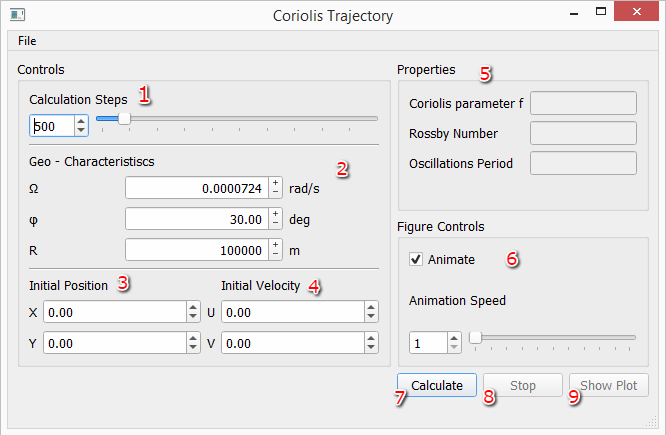
\includegraphics[scale=0.8]{coriolis-gui}
\caption{Γραφική διεπαφή χρήστη του λογισμικού \lat{"Coriolis Trajectory"}.}
\label{fig:coriolis-gui}
\end{figure}
Στο σχήμα \ref{fig:coriolis-gui} φαίνεται το κύριο παράθυρο του λογισμικού. Στην αριστερή μεριά του παραθύρου ο χρήστης έχει τη δυνατότητα να παραμετροποιήσει τη λύση, ενώ στη δεξιά πλευρά εμφανίζονται μερικές χρήσιμες χαρακτηριστικές τιμές καθώς και οι λειτουργίες ελέγχου των παραγώμενων γραφημάτων. Κατά σειρά αρίθμησης
\begin{enumerate}
\item Ορισμός του αριθμού βημάτων επίλυσης
\item Χαρακτηριστικά που αφορούν το επίπεδο επίλυσης
	\begin{itemize}
	\item [\textbf{Ω}] O ρυθμός περιστροφής του επιπέδου, $7.24e^{-5} rad/s$ για το ρυθμό περιστροφής της γης γύρω από τον άξονά της
	\item [\textbf{φ}] Το γεωγραφικό πλάτος εξέλιξης του φαινομένου. Επιτρέπονται τιμές από $-90\degree$ έως $90\degree$. Για τα σωματίδια που εκτελούν κίνηση στον ισημερινό, δηλαδή για $φ=90\degree$ δεν ορίζεται η δύναμη \cor και το πρόγραμμα ειδοποιεί το χρήστη με σχετικό μήνυμα. Ανάλογα με το πρόσημο $\pm$ του γεωγραφικού πλάτους, στο βόρειο ή νότιο ημισφαίριο, το λογισμικό επιλέγει αυτόματα το πρόσημο της γωνιακής ταχύτητας, έτσι ώστε τα αποτελέσματα να έχουν και φυσική υπόσταση.
	\item[\textbf{\lat{R}}] Η ακτίνα του περιστρεφόμενου δακτυλίου. Προτείνεται να μην ξεπερνάει τα 100\lat{km}, καθώς αυτή είναι η οριακή τιμή για την οποία μπορούμε να θεωρήσουμε σταθερή τη συχνότητα \cor \lat{f}.
	\end{itemize}
\item Αρχική θέση του σωματιδίου
\item Αρχική ταχύτητα του σωματιδίου, στις συνιστώσες $(u, v)$ του καρτεσιανού επιπέδου
\item Χαρακτηριστικά της κίνησης
	\begin{description}[style=nextline]
	\item[\small\textbf{Παράμετρος \cor \lat{f}}] Η συχνότητα \cor
	\item[\small\textbf{Αριθμός \ros}] Ο αριθμός \ros, χαρακτηριστικός του φαινομένου.
	\item[\small\textbf{Συχνότητα αδρανειακών ταλαντώσεων}] Η συχνότητα της ταλάντωσης που εκτελεί ένα σωματίδιο ρευστού, κατά την οποία οι αδρανειακές δυνάμεις που του ασκούνται εξισορροπούνται πλήρως από τη δύναμη \cor.
	\end{description}
\item Επιλογή για την απεικόνιση των αποτελεσμάτων σε μορφή βίντεο (\lat{animation}).
\item Το βασικό κουμπί εκτέλεσης του προγράμματος. Ελέγχει τα δεδομένα και στο τέλος των υπολογισμών εμφανίζει τη γραφική παράσταση του αποτελέσματος
\item Στην περίπτωση που οι υπολογισμοί διαρκούν πολύ ώρα, δίνεται στο χρήστη δυνατότητα τερματισμού
\item Εμφανίζει τη γραφική παράσταση, σύμφωνα με τις επιλογές του χρήστη στο $(6)$, χωρίς την επανέναρξη του υπολογισμού
\end{enumerate}

Πρέπει να σημειωθεί ότι έχει υλοποιηθεί προγραμματισμός που κάνει χρήση παραπάνω τους ενός πυρήνα του επεξεργαστή, δίνοντας στο χρήστη τη δυνατότητα να υπολογίσει και να εμφανίσει ταυτόχρονα πολλά διαφορετικά σενάρια επίλυσης.

\subsubsection{Παράθυρο γραφικής παράστασης}
\begin{figure}
\label{fig:cor-graph}
\centering
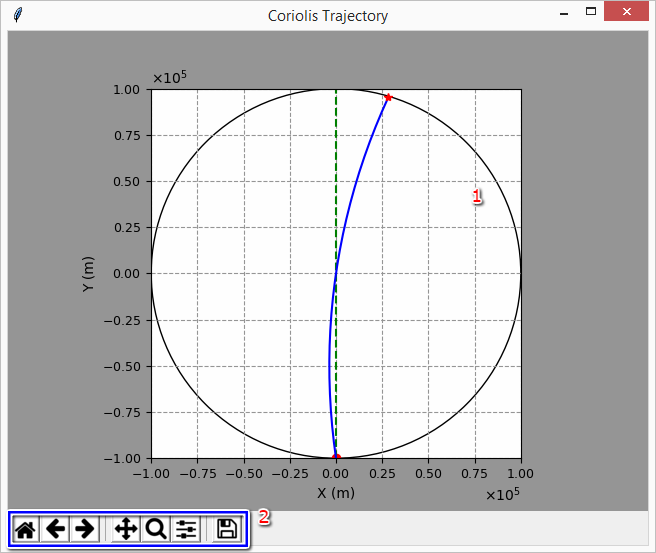
\includegraphics[scale=0.7]{cor-graph}
\caption{Παράθυρο γραφικής παράστασης του λογισμικού \lat{"Coriolis Trajectory"}}
\end{figure}
Το δεύτερο παράθυρο του λογισμικού εμφανίζει γραφικά τα αποτελέσματα των υπολογισμών. Τα αποτελέσματα εμφανίζονται είτε με τη μορφή βίντεο, είτε σταθερά, αναλόγως με την επιλογή του χρήστη. Ακόμα, υπάρχει η δυνατότητα εξαγωγής και αποθήκευσης του γραφήματος σε ένα αρχείο εικόνας. Στο παράθυρο φαίνονται
\begin{enumerate}
\item Το κυρίως γράφημα
\begin{description}[style=nextline]
\item[\small{Μαύρη γραμμή}] Τα όρια του περιστρεφόμενου κυκλικού δίσκου
\item[\small{Πράσινη γραμμή}] Η τροχιά του σωματιδίου στο αδρανειακό σύστημα αναφοράς
\item[\small{Μπλε γραμμή}] Η τροχιά του σωματιδίου στο περιστρεφόμενο σύστημα αναφοράς
\item[\small{Κόκκινος κύκλος}] Η αρχική θέση του σωματιδίου
\item[\small{Κόκκινο αστέρι}] Η τελική θέση του σωματιδίου
\end{description}
\item Επιλογές για την παραμετροποίηση της εμφάνισης του γραφήματος, καθώς και αποθήκευσής του σε αρχείο εικόνας
\end{enumerate}

\subsection{Αποτελέσματα και Σχολιασμός}
Το λογισμικό επιστρέφει στο χρήστη μερικές χρήσιμες τιμές, ώστε αυτός να μπορεί να αξιολογήσει τα αποτελέσματα. Μία από αυτές είναι ο αριθμός \ros. Ο αριθμός αυτός αποτελεί τον αδιάστατο λόγο των αδρανειακών δυνάμεων προς τις δυνάμεις \lat{Coriolis}. 

Η τάξη μεγέθους αυτού του αριθμού δηλώνει κατά πόσο η τροχιά ενός σωματιδίου επηρεάζεται από την περιστροφή του συστήματος συντεταγμένων, όπως για παράδειγμα όταν ένα σωματιδίου που εκτελεί μία κίνηση επηρεάζεται από την περιστροφή της γης γύρω από τον άξονα της. Όταν η τιμή του αριθμού \lat{Rossby} είναι αρκετά μεγάλη, δηλαδή οι αδρανειακές δυνάμεις υπερισχύουν των δυνάμεων \lat{Coriolis} και το σύστημα έρχεται σε κυκλοστροφική ισορροπία, φαίνεται ότι η τροχιά του σωματιδίου δεν επηρεάζεται από την περιστροφή του συστήματος. \textbf{[ΑΝΑΦΟΡΑ ΕΙΚΟΝΑΣ ΕΔΩ]}. Στην αντίθετη περίπτωση που ο αριθμός \ros είναι μικρός, το σύστημα έρχεται σε γεωστροφική ισορροπία και οι δυνάμεις \cor υπερισχύουν των αδρανειακών δυνάμεων, η τροχιά του σωματιδίου επηρεάζεται σε μεγάλο βαθμό από την περιστροφή του συστήματος συντεταγμένων. \textbf{[ΑΝΑΦΟΡΑ ΕΙΚΟΝΑΣ ΕΔΩ]}

\subsubsection{Αδρανειακές Ταλαντώσεις}
Οι αδρανειακές ταλαντώσεις είναι η πιο απλή μορφή κίνησης στη γη, η οποία επηρεάζεται από τη χρονική της διάρκεια. Στην πραγματικότητα, τέτοιου είδους κίνηση δεν εμφανίζεται μόνο στην περίπτωση της περιστρεφόμενης γης. Ένα απλό παράδειγμα για την κατανόηση των δυνάμεων που επηρεάζουν τέτοιες κινήσεις, είναι το παράδειγμα του περιστρεφόμενου παραβολικού δίσκου.
\begin{figure}[ht]
	\centering
	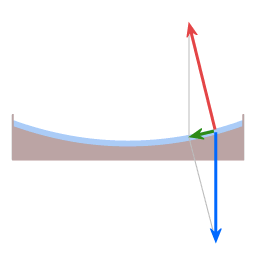
\includegraphics[scale=0.7]{images/coriolis-parabolic-disk.png}
	\caption{Οι δυνάμεις στο πείραμα του περιστρεφόμενου παραβολικού δίσκου. \lat{\cite{parbolicDisk}}}
	\label{fig:coriolis-parbolic-disk}
\end{figure}

Στο πείραμα του περιστρεφόμενου παραβολικού δίσκου, Σχήμα \ref{fig:coriolis-parbolic-disk}, αφήνεται ένα σώμα να εκτελέσει μία ελεύθερη ταλάντωση στην άτριβη επιφάνεια. Η δύναμη επαναφοράς είναι ανάλογη της απόστασης από το κέντρο της παραβολής. Παρατηρώντας αυτήν την κίνηση από ένα αδρανειακό σύστημα, φαίνεται ότι το σώμα εκτελεί μία ελλειπτική κίνηση, η οποία ονομάζεται αδρανειακή ταλάντωση.

Στο φυσικό κόσμο, η δύναμη επαναφοράς είναι η φαινόμενη δύναμη \lat{Coriolis}. Η περιστροφή της γης επηρεάζει τις κινήσεις που είναι πολύ "αργές" σε σχέση με την περιστροφή της, όπως τα κύματα με μεγάλο μήκος και μικρή συχνότητα, τα αδρανειακά κύματα (\lat{inertial waves}).

Τα αδρανειακά κύματα είναι εγκάρσια μηχανικά κύματα, που σε αντίθεση με τα επιφανειακά, λαμβάνουν χώρα στα εσωτερικά στρώματα ενός ρευστού. Τέτοια κύματα εμφανίζονται συνήθως στην ατμόσφαιρα της γης, παραδείγματος χάρη τα κύματα \lat{Rossby} και τα γεωστροφικά ρεύματα.

Τέτοια κύματα συναντώνται και στον ωκεανό, με τη μορφή κυμάτων \lat{Poincare}. Κύμα \lat{Poincare} μπορεί να θεωρηθεί και η διάδοση της παλίρροιας, καθώς και όλα τα κύματα ρηχού στρώματος (\lat{SWW}), μακριά από τη στεριά.

Η συχνότητα των επιφανειακών κυμάτων \lat{Poincare} είναι ίδια με την συχνότητα κυμάτων ρηχού στρώματος, με την προσθήκη της παραμέτρου \lat{Coriolis}, \lat{f}.
\begin{equation}
	ω = \sqrt{f^2+gHk^2}
\end{equation}

Η ταχύτητα ομάδας (\lat{Group velocity}) είναι
\begin{equation}
	C_g = \dfrac{\partial{ω}}{\partial{k}} = \dfrac{gHk}{\sqrt{f^2+gHk^2}}
\end{equation}

Όταν $f \rightarrow 0$ ή $k^2 \gg \dfrac{f^2}{gH}$ τότε $C_g=\sqrt{gH}$ και το κύμα συμπεριφέρεται σαν απλό κύμα ρηχού στρώματος, χωρίς της επιρροή της περιστροφής της γης. Στην αντίθετη περίπτωση, όπου $k \rightarrow 0$ τότε $C_g = 0$, δεν υπάρχει διάδοση του κύματος και εκτελείται μία αδρανειακή ταλάντωση.

Η επίλυση στη μία διάσταση ενός κύματος \lat{Poincare} είναι
\begin{align}
	u &= \dfrac{ω}{kH}H_0\cos(kx-ωt) \\
	v &= \dfrac{f}{kH}H_0\sin(kx-ωt)
\end{align}

Εύκολα, μπορούμε να υπολογίσουμε πότε η περιστροφή της γης είναι σημαντική. Η χαρακτηριστική κλίμακα μήκους είναι
\begin{equation}
	L \rightarrow 1/k \Rightarrow L_R = \dfrac{\sqrt{gH}}{H}
\end{equation}
και ονομάζεται \textbf{\lat{Rossby radius of deformation}}. Για μήκος μικρότερο από την τιμή της κλίμακας η περιστροφή δεν επηρεάζει την κίνηση.

\subsubsection{Υπολογισμός του αριθμού \ros}
Ο αριθμός \ros αποτελεί έναν αδιάστατο αριθμό χαρακτηριστικό για το κάθε πρόβλημα, ο δε υπολογισμός του είναι εύκολος κάνοντας χρήση και ανάλυση των εγγενών κλιμάκων του προβλήματος.

Έχοντας ως βασική κλίμακα το \textbf{χρόνο}, μπορεί να προσδιοριστεί τόσο ο χρόνος που απαιτείται ώστε ένα σημείο επάνω στο όριο του κύκλου που περιγράφει το περιστρεφόμενο σύστημα αναφοράς να κάνει μία πλήρη περιστροφή, όσο και ο χρόνος που απαιτείται ώστε ένα σωματίδιο, που εκτελεί την εξεταζόμενη κίνηση, να διαγράψει μία διαμετρική πορεία.

Ο χρόνος που απαιτείται ώστε ένα σημείο του κύκλου να διαγράψει μία πλήρη περιστροφή είναι
\begin{equation}
\label{eq:t_r}
t_{R}=\frac{2\pi}{\Omega}
\end{equation}
ενώ ο χρόνος που απαιτείται ώστε ένα σωματίδιο να εκτελέσει ευθύγραμμη ομαλή κίνηση και να διαγράψει απόσταση ίση με τη διάμετρο του κυκλικού δίσκου είναι
\begin{equation}
\label{eq:t_i}
t_{I}=\frac{2R}{\mathbb{V}}
\end{equation}
όπου $Ω$ είναι η σταθερή γωνιακή ταχύτητα του κυκλικού δίσκου, $R$ η διάμετρός του και $\mathbb{V}$ η χαρακτηριστική ταχύτητα της ευθύγραμμης κίνησης.

Συνδυάζοντας τις \ref{eq:t_r} και \ref{eq:t_i}, που έχουν ως κλίμακα το χρόνο, $[T]$, προκύπτει ο αδιάστατος αριθμός \ros
\begin{equation}
\label{eq:ro}
Ro = \dfrac{t_{R}}{t_{I}} \; \Rightarrow \;
Ro = \dfrac{\dfrac{2π}{Ω}}{\dfrac{2R}{\mathbb{V}}}
\end{equation}

Κάνοντας τις απλοποιήσεις και απαλοίφοντας το σταθερό όρο $π$, προκύπτει ο αριθμός \ros που χρησιμοποιήθηκε στο λογισμικό
\begin{equation}
Ro = \dfrac{\mathbb{V}}{ΩR}
\end{equation}
	\cleardoublepage
	\section{Μοντελοποίηση κυκλοφορίας σε ανοιχτό από το ένα άκρο κόλπο}
		Στο κεφάλαιο αυτό παρουσιάζεται η μοντελοποίηση της κυκλοφορίας σε έναν εξιδανικευμένο κόλπο, όπου το ένα άκρο του είναι ανοιχτό (\lat{open-sea-boundary}), ενώ τα υπόλοιπα κλειστά (στεριά).

Ο κόλπος έχει εξιναδικευτεί ώστε να έχει κάτοψη ορθογωνίου, με σταθερό βάθος και άτριβο πυθμένα. Το μοντέλο περιγράφει τη διάδοση ενός παλιρροϊκού κύματος από την ανοιχτή θάλασσα και το κλειστό άκρο, στο οποίο προσπίπτει το κύμα, προκαλεί τέλεια ανάκλαση.
\subsection{Παλίρροια και παλιρροϊκή κυκλοφορία}
Το φαινόμενο της παλίρροιας αναφέρεται στην περιοδική κίνηση του νερού της θάλασσας και οφείλεται στην διαφορά των ελκτικών δυνάμεων του Ηλίου και της Σελήνης, στις διάφορες φάσεις της.
Ως παλίρροια αναφέρεται η περιοδική ανύψωση και ταπείνωση της στάθμης της θάλασσας και συνοδεύεται από το παλλιροϊκό ρεύμα, δηλαδή την οριζόντια κίνηση του νερού. Και οι δύο κινήσεις αποτελούν μέρη του ίδιου φαινομένου.

Η περιοδική ανύψωση και ταπείνωση της στάθμης της θαλάσσας είναι επί της ουσίας ένα μακρύ κύμα το οποίο διαδίδεται. Η περίοδος ενός τέτοιου κύματος είναι συγκρίσιμη με το χρόνο περιστροφής της γης, αφού η παλίρροια μπορεί να έχει περίοδο 6, 12, ακόμα και 24 ώρες, οπότε επηρεάζεται από αυτή. Για αυτό στις εξισώσεις ορμής είναι απαραίτητη η προσθήκη του όρου της δύναμης \cor, εφόσον το φαινόμενο εξελίσεται σε μεταξύ διαφορετικών γεωγραφικών πλατών.

Ένα μακρύ κύμα περιγράφεται από την εξίσωση 
\begin{equation}
    η = \dfrac{H}{2}\cos{(kx-ωt)}
\end{equation}
όπου $Η$ το πλάτος κύματος, $k=\dfrac{2π}{L}$ o κυματαριθμός, $ω=\dfrac{2π}{T}$ η κυκλική συχνότητα, $L$ το μήκος κύματος και $T$ η περίοδος.

\subsection{Εξισώσεις ρηχού στρώματος - \lat{SWE}}
Πολλοί τύποι ροών μπορούν να χαρακτηριστούν ως "ροές ρηχού στρώματος". Με τον όρο ροή δεν είναι απαραίτητη η παραπομπή μόνο σε ροή ύδατος. Ροές όπως η κυκλοφορία ατμοσφαιρικών μαζών, η παλίρροια, πλημυρικά ρέματα, η παράκτια κυκλοφορία, τα \lat{tsunamis} κ.ά., μπορούν να περιγραφούν με τις εξισώσεις ρηχού στρώματος. Το βασικό χαρακτηριστικό τέτοιων ροών είναι ότι η κλίμακα του βάθους είναι πολύ μικρότερη από την οριζόντια χαρακτηριστική κλίμακα.
\begin{equation}
    \dfrac{h}{L} \ll 1
\end{equation}

Επομένως το αν θα εμπίπτει μία ροή στην κατηγορία εξισώσεων ρηχού στρώματος έχει σχέση με τις γεωμετρικές διαστάσεις της ίδιας της ροής και όχι του ρευστού όγκου που εξετάζεται. Για παράδειγμα η παλιρροϊκή ροή σε έναν ωκεανό περιγράφεται από τις εξισώσεις ρηχού στρώματος, όμως η ανεμογενής κυκλοφορία σε έναν ταμιευτήρα όχι, παρόλο που το βάθος του ταμιευτήρα είναι πολύ μικρό.

Στο μοντέλο του ρηχού στρώματος υπεισέρχεται η βασική απλοποιήση ότι η κατακόρυφη συνιστώσα της ταχύτητας, οπότε και της επιτάχυνσης είναι αμελητέες. Έτσι, η κατακόρυφη εξίσωση ορμής αποτελείται από υδροστατική ισορροπία.

Το σύστημα των διαφορικών εξισώσεων που περιγράφουν το πρόβλημα είναι οι εξισώσεις ορμής \lat{Navier - Stokes} και η εξίσωση συνέχειας. Ύστερα από ανάλυση της κλίμακας κάθε όρου των εξισώσεων και απαλοιφής των ασήμαντων, λόγω κλίμακας, όρων οι εξισώσεις ορμής για τους άξονες $x$, $y$, $z$ είναι αντίστοιχα
\begin{align}
    \dfrac{\partial{u}}{\partial{t}} + u\dfrac{\partial{u}}{\partial{x}} + v\dfrac{\partial{u}}{\partial{y}} + w\dfrac{\partial{u}}{\partial{z}} &= fv-\dfrac{1}{ρ}\dfrac{\partial{p}}{\partial{x}} + \dfrac{\partial}{\partial{z}}\left(ε_z\dfrac{\partial{u}}{\partial{z}}\right) \\
    \dfrac{\partial{v}}{\partial{t}} + u\dfrac{\partial{v}}{\partial{x}} + v\dfrac{\partial{v}}{\partial{y}} + w\dfrac{\partial{v}}{\partial{z}} &= fv-\dfrac{1}{ρ}\dfrac{\partial{p}}{\partial{y}} + \dfrac{\partial}{\partial{z}}\left(ε_z\dfrac{\partial{v}}{\partial{z}}\right) \\
    0 &= -\dfrac{1}{ρ}\dfrac{\partial{p}}{\partial{z}} - g
\end{align}
Το σύστημα συμπληρώνεται με την εξίσωση συνέχειας
\begin{equation}
    \dfrac{\partial{u}}{\partial{x}} + \dfrac{\partial{v}}{\partial{y}} + \dfrac{\partial{w}}{\partial{z}} = 0
\end{equation}

Η ύπαρξη ελεύθερης επιφάνειας του νερού εισάγει έναν ακόμα άγνωστο στο πρόβλημα της κυκλοφορίας. Η ανάπτυξη οποιουδήποτε ρεύματος συνεπάγεται τη μετατόπιση της ελεύθερης επιφάνειας από τη θέση ισορροπίας της, με αποτέλεσμα το πεδίο ορισμού της λύσης να είναι άγνωστο.

Ένας τρόπος αντιμετώσης αυτού του προβλήματος είναι να δημιουργήσουμε μία εξίσωση που να περιγράφει την θέση της ελεύθερης επιφάνειας κάθε χρονική στιγμή. Για το λόγο αυτό ολοκληρώνεται ως προς το βάθος η εξίσωση συνέχειας.

Έστω ότι με $ζ(t, x, y)$ συμβολίζεται το τοπικό βάθος της υδάτινης μάζας. Τότε η ολοκληρωμένη ως προς το βάθος εξίσωση συνέχειας δίνει
\begin{equation}
    \dfrac{\partial{ζ}}{\partial{t}} + \dfrac{\partial}{\partial{x}}\left(ζU\right) + \dfrac{\partial}{\partial{y}}\left(ζV\right) = 0 \label{eq:int-cont}
\end{equation}
όπου $U$ και $V$ οι μέσες ως προς το βάθος τιμές των $u$ και $v$ αντίστοιχα.

Ακόμα ολοκληρώνοντας την υδροστατική εξίσωση ως προς το βάθος, καταλήγουμε
\begin{align}
    -\dfrac{1}{ρ}\dfrac{\partial{p}}{\partial{x}} &= -g\dfrac{\partial{η}}{\partial{x}}-\dfrac{1}{ρ}\dfrac{\partial{p_α}}{\partial{x}} \\
    -\dfrac{1}{ρ}\dfrac{\partial{p}}{\partial{y}} &= -g\dfrac{\partial{η}}{\partial{y}}-\dfrac{1}{ρ}\dfrac{\partial{p_α}}{\partial{y}}
\end{align}

Μετά από τις κατάλληλες αντικαταστάσεις στο αρχικό σύστημα καταλήγουμε στις εξισώσεις ορμής, που μαζί με την ολοκληρωμένη ως προς το βάθος εξίσωση συνέχειας, αποτελούν τη βάση του μοντέλου ρηχού στρώματος
\begin{align}
    \dfrac{\partial{u}}{\partial{t}} + u\dfrac{\partial{u}}{\partial{x}} + v\dfrac{\partial{u}}{\partial{y}} + w\dfrac{\partial{u}}{\partial{z}} &= fv-g\dfrac{\partial{η}}{\partial{x}}-\dfrac{1}{ρ}\dfrac{\partial{p_α}}{\partial{x}} + \dfrac{\partial}{\partial{z}}\left(ε_z\dfrac{\partial{u}}{\partial{z}}\right) \label{eq:u-mom-non}\\
    \dfrac{\partial{v}}{\partial{t}} + u\dfrac{\partial{v}}{\partial{x}} + v\dfrac{\partial{v}}{\partial{y}} + w\dfrac{\partial{v}}{\partial{z}} &= fv-g\dfrac{\partial{η}}{\partial{y}}-\dfrac{1}{ρ}\dfrac{\partial{p_α}}{\partial{y}} + \dfrac{\partial}{\partial{z}}\left(ε_z\dfrac{\partial{v}}{\partial{z}}\right) \label{eq:v-mom-non}
\end{align}

\subsubsection{Τελικό μοντέλο}
Το μοντέλο που εξετάζεται στην παρούσα διπλωματική είναι αρκετά απλοποιημένο και δεν είναι απαραίτητη η χρήση όλων των όρων των εξισώσεων. Οι μη γραμμικοί όροι στις παραπάνω εξισώσεις μεταθέτουν μεν την ορμή, χωρίς όμως να μεταβάλλουν την ολική τιμή της. Καθώς η κυκλοφορία καθορίζεται από την ισορροπία των δυνάμεων, η μορφή της διατηρείται και στη γραμμικοποιημένη μορφή των εξισώσεων. Ακόμα, θεωρούμε ότι ο πυθμένας του κόλπου είναι άτριβος, η ατμοσφαιρική πίεση είναι σταθερή σε όλη την κάτοψη, καθώς και η εξέλιξη του φαινομένου γίνεται στο ίδιο γεωγραφικό πλάτος, με αποτέλεσμα η δύναμη \cor να μην επηρεάζει τη λύση.

Με βάση όλες αυτές τις παραδοχές, οι εξισώσεις \ref{eq:u-mom-non}, \ref{eq:v-mom-non} και \ref{eq:int-cont} γίνονται
\begin{align}
    \dfrac{\partial{u}}{\partial{t}} &= -g\dfrac{\partial{η}}{\partial{x}} \label{eq:u} \\
    \dfrac{\partial{v}}{\partial{t}} &= -g\dfrac{\partial{η}}{\partial{y}} \label{eq:v}
\end{align}
\begin{equation}
    \dfrac{\partial{η}}{\partial{t}} + h\dfrac{\partial{U}}{\partial{x}} + h\dfrac{\partial{V}}{\partial{y}} = 0 \label{eq:int-cont-new}
\end{equation}

Μετά από παραγώγιση των εξισώσεων \ref{eq:u} και \ref{eq:v} ως προς $x$ και $y$ αντίστοιχα και παραγώγιση της \ref{eq:int-cont-new} ως προς $t$, καταλήγουμε στην εξίσωση κύματος
\begin{equation}
    \dfrac{\partial^2{η}}{\partial{t}^2} = gh\left( \dfrac{\partial^2{η}}{\partial{x}^2} + \dfrac{\partial^2{η}}{\partial{y}^2} \right) \label{eq:wave}
\end{equation}
η οποία είναι μια υπερβολική διαφορική εξίσωση της μορφής $\dfrac{\partial^2{\vec{u}}}{\partial{t}^2}=c^2 \nabla^2 \vec{u}$, με $\vec{u} = \vec{u}(x_1, x_2, ... , x_n)$ βαθμωτή συνάρτηση της οποίας οι τιμές αποτελούν τη μετατόπιση ενός κύματος. Γίνεται αμέσως φανερό ότι η ταχύτητα του κύματος είναι 
\begin{equation}
    c=\sqrt{gh} \label{eq:celerity}
\end{equation}

\subsection{Διακριτοποίση των εξισώσεων}
Η αριθμητική επίλυση του προβλήματος γίνεται διακριτοποιώντας τις εξισώσεις (\ref{eq:u}), (\ref{eq:v}) και (\ref{eq:wave}). Επηλέχθηκε να γίνει χρήση της μεθόδου \textit{πεπερασμένων διαφορών}, έναντι της μεθόδου πεπερασμένων στοιχείων, προς χάρη της απλότητάς της. Βασιζόμενοι στη λογική της απλότητας χρησιμοποιήθηκε ένα ρητό σχήμα, διακριτοποιώντας το χρόνο με πρόσω διαφορές και το χώρο με κεντρικές, όπως συνιθίζεται σε φαινόμενα μεταφοράς.

Έτσι η διακριτοποιημένη μορφή της εξίσωση κύματος (\ref{eq:wave}) είναι
\begin{equation}
    η_{i,j}^{n+1} = 2 η_{i,j}^{n} - η_{i,j}^{n-1} + \dfrac{c^2 Δt^2}{Δx^2}\left( η_{i+1,j}^{n} - 2 η_{i,j}^{n} + η_{i-1,j}^{n}\right) + \dfrac{c^2 Δt^2}{Δy^2}\left( η_{i,j+1}^{n} - 2 η_{i,j}^{n} + η_{i,j+1}^{n}\right) \label{eq:dis:wave-1}
\end{equation}
όπου $c$ είναι η ταχύτητα κύματος, όπως υπολογίζεται στην εξίσωση (\ref{eq:celerity}).

Για λόγους ευπαρουσίασης της εξίσωσης (\ref{eq:dis:wave-1}), συμβολίζουμε ως
\begin{align}
    H_{x} &= η_{i+1,j}^{n} - 2 η_{i,j}^{n} + η_{i-1,j}^{n} \\
    H_{y} &= η_{i,j+1}^{n} - 2 η_{i,j}^{n} + η_{i,j+1}^{n} \\
    C_{xs} &= \dfrac{c^2 Δt^2}{Δx^2} \label{eq:cour-x-s}\\
    C_{ys} &= \dfrac{c^2 Δt^2}{Δy^2} \label{eq:cour-y-s}
\end{align}
οπότε η (\ref{eq:dis:wave-1}) γίνεται
\begin{equation}
    η_{i,j}^{n+1} = 2 η_{i,j}^{n} - η_{i,j}^{n-1} + C_{xs} H_{x} + C_{ys} H_{y}
    \label{eq:dis:wave}
\end{equation}
Οι αριθμοί (\ref{eq:cour-x-s}) και (\ref{eq:cour-x-s}), είναι το τετράγωνο του αριθμού \lat{Courant} για κάθε μία από τις δύο διευθύνσεις.

Για τη διακριτοποίηση των διαφορικών εξισώσεων της ταχύτητας (\ref{eq:u}) και (\ref{eq:v}) έγινε χρήση του ίδιου σχήματος, επομένως οι διακριτοποιημένες εξισώσεις, χρησιμοποιώντας τον παραπάνω συμβολισμό είναι
\begin{align}
    u_{i,j}^{n+1} &= u_{i,j}^{n} - g \dfrac{Δt}{Δx^2}H_x \label{eq:dis:u}\\
    v_{i,j}^{n+1} &= v_{i,j}^{n} - g \dfrac{Δt}{Δy^2}H_y \label{eq:dis:v}
\end{align} 
\subsubsection{Ευστάθεια της λύσης}
Όπως κάθε ρητό σχήμα επίλυσης, έτσι και αυτό που αναπτύχθηκε παραπάνω, είναι απαραίτητη η ύπαρξη μιας σχέσης που συνδέει το χρονικό βήμα, με το χωρικό βήμα.

Σύμφωνα με τον περιορισμό \lat{Courant-Friedrichs–Lewy} (\textbf{\lat{CFL condition}}) το χρονικό βήμα πρέπει να έχει τιμή μικρότερη από ένα συγκεκριμένο χρονικό διάστημα ώστε η αριθμητική λύση μιας υπερβολικής διαφορικής εξίσωσης να συγκλίνει.

Η μορφή του περιορισμού \lat{CFL} έχει σχέση με το πεδίο ορισμού της εξίσωσης που πρόκειται να λυθεί. Στο πρόβλημα της κυκλοφορίας σε ένα κόλπο, η επίλυση γίνεται στις δύο οριζόντιες διαστάσεις $x$, $y$ και η υπόθεση είναι 
\begin{equation}
    C = c Δt \dfrac{Δx + Δy}{Δx Δy}
\end{equation}
που προέκυψε από πρόσθεση του αριθμού \lat{Courant} για κάθε διεύθυνση.

Από φυσική άποψη, ο περιορισμός \lat{CFL} αναφέρεται στο γεγονός ότι το χρονικό βήμα πρέπει να είναι μικρότερο από το χρόνο που χρειάζεται το κύμα για να διασχίσει ένα χωρικό βήμα. Όταν η επίλυση του κύματος γίνεται στη μία διάσταση, αρκεί $ C \le 1$. Στην περίπτωση όμως που η επίλυση γίνεται στις δύο διαστάσεις, όπως στην παρούσα διπλωματική εργασία, ο περιορισμός γίνεται πιο αυστηρός και πρέπει $ C \le \dfrac{1}{\sqrt{2}} $. Η αυστηρότητα του περιορισμού έγγυται στο γεγονός ότι όταν ένα κύμα κινείται υπό γωνία στο πλέγμα επίλυσης πρέπει να διανύσει τη διαγώνια απόσταση ενός κελιού. Αυτό συχνά αναφέρεται και ως \textit{αριθμητικό ιξώδες} ή \textit{αριθμητική διάχυση}.

Με βάση λοιπόν τα παραπάνω, υπάρχει ένας περιορισμός για το μέγιστο χρονικό βήμα που είναι δυνατό να χρησιμοποιηθεί κατά την επίλυση και αυτό έχει άμεση σχέση με το χωρικό βήμα που επιλέγεται σε κάθε διεύθυνση. Επομένως, με γνωστό $Δx$ και $Δy$, το χρονικό βήμα υπολογίζεται
\begin{equation}
    Δt = \sqrt{2}\dfrac{ΔxΔy}{Δx+Δy}
    \label{eq:timestep}
\end{equation}

\subsection{Διαδικασία επίλυσης}
Η επίλυση του προβλήματος γίνεται σε τρία βασικά στάδια, την αρχικοποίηση των μεταβλητών με τα δεδομένα του προβλήματος, τους βασικούς υπολογισμούς και, τέλος, την οπτικοποίηση των αποτελεσμάτων.

\subsubsection{Δεδομένα του προβλήματος}
Ο σκοπός αυτής της διπλωματικής, πέραν όσων αναφέρθηκαν στα προηγούμενα κεφάλαια, είναι να υπολογισθεί αριθμητικά και να παρουσιασθεί η κυκλοφορία σε έναν ανοιχτό από τη μία πλευρά κόλπο. Επιλέχθηκε οι διαστάσεις του κόλπου αυτού να είναι $25km$ σε πλάτος και $40km$ σε μήκος, ενώ το βάθος του να είναι σταθερό $50m$.

Τα ύδατα του κόλπου τη χρονική στιγμη $t=0$ βρίσκονται σε ηρεμία και η διαδικασία επίλυσης αρχίζει με τη διέγερση του ανοιχτού άκρου από ένα ημιτονοειδές κύμα πλάτους $40cm$. Πρέπει να τονισθεί ότι τα σημεία στο άκρο του κόλπου διεγείρονται όλα ταυτόχρονα, οπότε προσομοιάζεται ένα εξωτερικό κύμα που εισέχεται στον κόλπο κάθετα, όπως φαίνεται στο σχήμα \ref{fig:layout}.

\begin{figure}[]
	\centering
	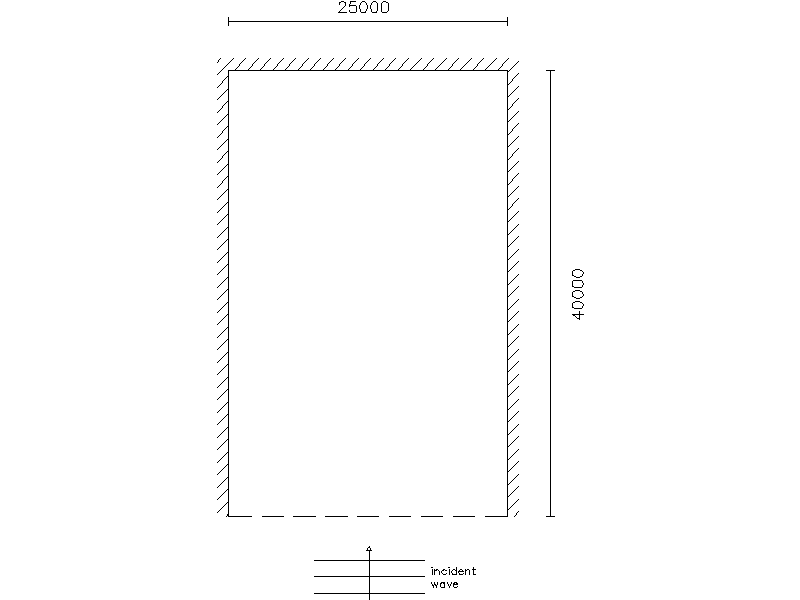
\includegraphics[scale=1.3]{images/layout.png}
	\caption{Κάτοψη του κόλπου. Με διακεκομένη γραμμή φαίνεται το ανοιχτό όριο.}
	\label{fig:layout}
\end{figure}

\begin{table}[h!]
    \centering
    \begin{tabular}{|l|r|l|r|}
        \hline
        \textbf{$L_x$} & $25km$ & \textbf{$T$} & $4000s$ \\
        \textbf{$L_y$} & $40km$ & \textbf{$A$} & $0.4m$ \\
        \textbf{$H$} & $50m$ & \textbf{$N_x$} & $50$ \\
        \textbf{$g$} & $9.807 m/s^2$ & \textbf{$N_y$} & $50$ \\
        \hline
    \end{tabular}
    \caption{Δεδομένα προβλήματος}
    \label{tab:in-data}
\end{table}

Στον Πίνακα \ref{tab:in-data} φαίνονται συγκεντρωμένα όλα τα δεδομένα του προβλήματος. Με $g$ συμβολίζεται η βαρυτική επιτάχυνση, ενώ με $N_x$ και $N_y$ ο αριθμός των κόμβων που επιλέχθηκαν για να δομήσουν το πλέγμα της επίλυσης. 

\subsubsection{Υπολογισμοί}
Οι υπολογισμοί για την επίλυση του προβλήματος διακρίνονται σε τρία στάδια.
\begin{itemize}
    \item Υπολογισμός χρονικού βήματος από την εξίσωση (\ref{eq:timestep})
    \item Για κάθε κόμβο του πλέγματος υπολογίζεται
    \begin{itemize}
        \item Η ανύψωση - ταπείνωση της ελεύθερης επιφάνειας $η$ από την εξίσωση (\ref{eq:dis:wave})
        \item Η οριζόντια ταχύτητα $u$ από την εξίσωση (\ref{eq:dis:u})
        \item Η κάθετη ταχύτητα $v$ από την εξίσωση (\ref{eq:dis:v})
    \end{itemize}
    \item Μεταβολή του χρόνου κατά $dt$ και επανάληψη του προηγούμενου βήματος
\end{itemize}

Ο προγραμματισμός της μεθόδου επίλυσης έγινε σε περιβάλλον \textit{Python} και το αντίστοιχο κομμάτι κώδικα φαίνεται στο παράρτημα \ref{sec:waterLevelPython} που υπολογίζεται η ανύψωση και ταπείνωση της ελεύθερης επιφάνειας, ενώ ο υπολογισμός της ταχύτητας φαίνεται στο παράρτημα \ref{sec:velocityPython}.

\subsubsection{Αρχικές και Συνοριακές συνθήκες}
Ο κόλπος πριν διεγερθεί από το εξωτερικό κύμα βρίσκεται σε κατάσταση ηρεμίας. Άρα οι αρχικές συνθήκες του προβλήματος είναι προφανές ότι θα είναι $0$ για την ανύψωση της ελεύθερης επιφάνειας, αλλά και για την ταχύτητα.
Η δυσκολία βρίσκεται στην εκλογή κατάλληλων συνοριακών συνθηκών, τέτοιων ώστε να προσομοιώνεται όσο το δυνατόν καλύτερα το πρόβλημα, με τους περιορισμούς που έχουμε θέσει.

Τα κλειστά άκρα του κόλπου (στεριά) προκαλούν πλήρη ανάκλαση των κυματισμών. Επομένως η επιλογή μία συνθήκης τύπου \lat{Neumann} είναι η πιο κατάλληλη. Για να υπάρχει πλήρης ανάκλαση των κυματισμών είναι απαραίτητο να μηδενίζεται η κλίση της ανύψωσης - ταπείνωσης της ελεύθερης επιφάνειας του νερού και όχι να μηδενίζεται η ίδια η τιμή της. Το ίδιο συμβαίνει και με την ταχύτητα. Επομένως οι συνοριακή συνθήκη για τα κλειστά άκρα του κόλπου είναι
\begin{align}
    \dfrac{\partial{η}}{\partial{x}} = \dfrac{\partial{η}}{\partial{y}} &= 0 \\
    \dfrac{\partial{u}}{\partial{x}} = \dfrac{\partial{v}}{\partial{y}} &= 0
\end{align}
Η εφαρμογή των παραπάνω συνθηκών έγινε προγραμματιστικά με την εισαγωγή \textit{κόμβων-φαντασμάτων} όπου η τιμή τους αυτόματα παίρνει την τιμή του προηγούμενου κόμβου. Έτσι, η διαφορά τους είναι $0$ και η κλίση του διανύσματος είναι, επίσης, $0$.

Για το ανοιχτό άκρο η εκλογή μια συνοριακής συνθήκης είναι πιο περίπλοκη, γιατί υπάρχει το προσπίπτων κύμα που μπαίνει στον κόλπο, αλλά και τα ανακλανόμενα κύματα που εξέρχονται από τον κόλπο. Το πρόβλημα είναι δυνατόν να λυθεί με χρήση της \textit{ελεύθερης ακτινοβολίας} που προτείνει ο \cite{koutitas}.
\begin{equation}
    \dfrac{\partial{ζ_r}}{\partial{t}} + \sqrt{gh} \dfrac{\partial{ζ_r}}{\partial{y}} = 0 
\end{equation}
η διακριτοποιήση της οποίας ακολουθεί το ίδιο σχήμα με τη διακριτοποίηση της ανύψωσης της ελεύθερης επιφάνειας, με πρόσω διαφορές στο χρόνο και κεντρικές διαφορές στο χώρο.
\begin{equation}
    ζ_{i,j}^{n+1} = 2 ζ_{i,j}^{n} - ζ_{i,j}^{n-1} + gh\dfrac{Δt^2}{2Δy^2}\left( ζ_{i+1,j}^{n} - 2ζ_{i,j}^{n} + ζ_{i,j+1}^{n} \right)
\end{equation}

\subsection{Αποτελέσματα επίλυσης}
Η επίλυση έγινε για διάφορες χρονικές περιόδους και αριθμό κόμβων, ώστε να διαπιστωθεί η ευστάθεια της μεθόδου. Σαν οπτικό αποτέλεσμα για κάθε επίλυση, το πρόγραμμα επιστρέφει μία σειρά διαγραμμάτων. Μία κάτοψη του κόλπου που εμφανίζεται η ελεύθερη επιφάνεια μαζί με τα διανύσματα της ταχύτητας για την τελευταία χρονική στιγμή της επίλυσης και δύο διαγραμμάτα χρονοσειράς για τη μεταβολή της ελεύθερης επιφάνειας και τη μεταβολή της κατά $y$ ταχύτητας ενός συγκεκριμένου σημείου κατά τη διαδικασία επίλυσης, δηλαδή για όλες τις χρονικές στιγμές.

\begin{table}[h!]
    \begin{tabular}{|cccccc||ccc|}
    \hline
    \multicolumn{2}{|c}{\textbf{\begin{tabular}[c]{@{}l@{}}Κωδικός\\ Επίλυσης\end{tabular}}} & \textbf{\begin{tabular}[c]{@{}c@{}}Χρονική \\ διάρκεια\end{tabular}} & \textbf{$N_x$} & \textbf{$N_y$} & \textbf{Σημείο} & \textbf{$Δx$ [m]} & \textbf{$Δy$ [m]} & \textbf{$Δt$ [s]} \\ \hline
    \multirow{2}{*}{1} & a & 0.5d & 50 & 50 & μέσο αν. ορίου & 500 & 800 & 30 \\
     & b & 0.5d & 50 & 50 & κέντρο κόλπου & 500 & 800 & 30 \\
    \multirow{2}{*}{2} & a & 0.5d & 25 & 25 & μέσο αν. ορίου & 1000 & 1600 & 39\\
     & b & 0.5d & 25 & 25 & κέντρο κόλπου & 1000 & 1600 & 39 \\ \hline
    \multirow{2}{*}{3} & a & 1d & 50 & 50 & μέσο αν. ορίου & 500 & 800 & 30 \\
     & b & 1d & 50 & 50 & κέντρο κόλπου & 500 & 800 & 30 \\
    \multirow{2}{*}{4} & a & 1d & 25 & 25 & μέσο αν. ορίου & 1000 & 1600 & 39\\
     & b & 1d & 25 & 25 & κέντρο κόλπου & 1000 & 1600 & 39 \\ \hline
    \multirow{2}{*}{5} & a & 5d & 25 & 25 & μέσο αν. ορίου & 1000 & 1600 & 39 \\
    & b & 5d & 25 & 25 & κέντρο κόλπου & 1000 & 1600 & 39 \\ \hline
    \end{tabular}
    \caption{Διαφορετικές επιλύσεις του προβλήματος}
    \label{tab:result-table}
\end{table}
Στον Πίνακα \ref{tab:result-table} φαίνονται οι διαφορετικές επιλύσεις που έγιναν για χρόνους επίλυσης $12 h$, $1 day$ και $5 days$, με διαφορετικό αριθμό κόμβων κάθε φορά. Ακόμα φαίνονται τα υπολογισμένα μεγέθη $Δx$, $Δy$ και $Δt$.

\subsubsection{Διαγράμματα επιλύσεων}
\begin{figure}[h]
	\centering
	\subfigure[Διάγραμμα Ε.Ε. και ταχύτητας]{\label{fig:1aF}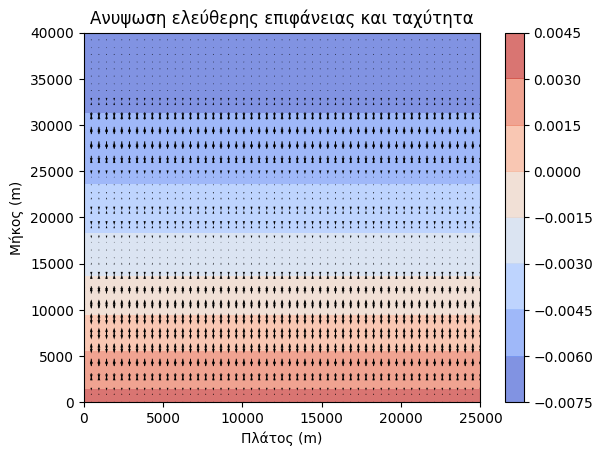
\includegraphics[scale=0.8]{1afinal_2d}}
	\subfigure[Διάγραμμα ταχύτητας σε κάτοψη]{\label{fig:1aV2d}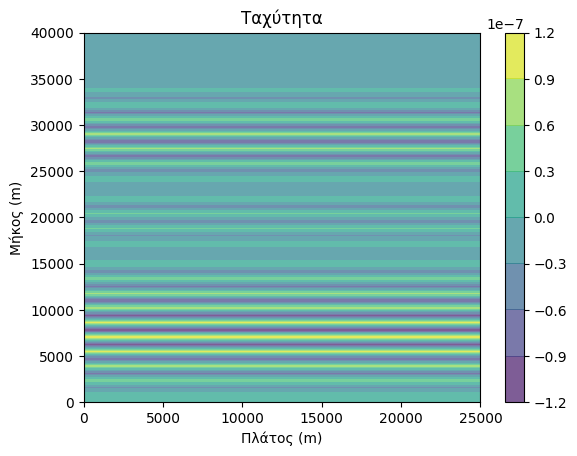
\includegraphics[scale=0.8]{1acontour}}
	\caption{Αποτελέσματα \lat{1a}}
\end{figure}
\begin{figure}[h]
	\centering
	\subfigure[Διάγραμμα Ε.Ε. και ταχύτητας]{\label{fig:1bF}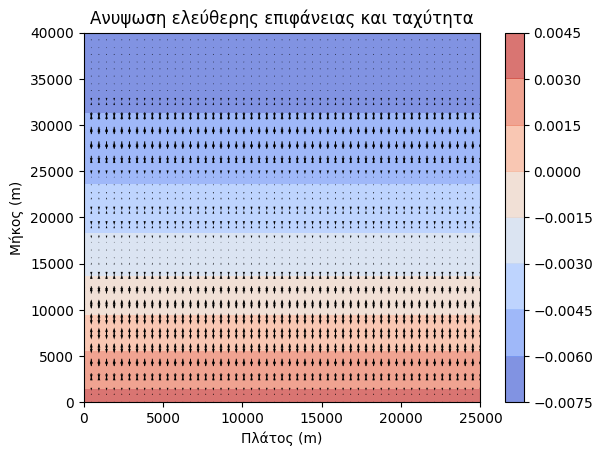
\includegraphics[scale=0.8]{1bfinal_2d}}
	\subfigure[Διάγραμμα ταχύτητας σε κάτοψη]{\label{fig:1bV2d}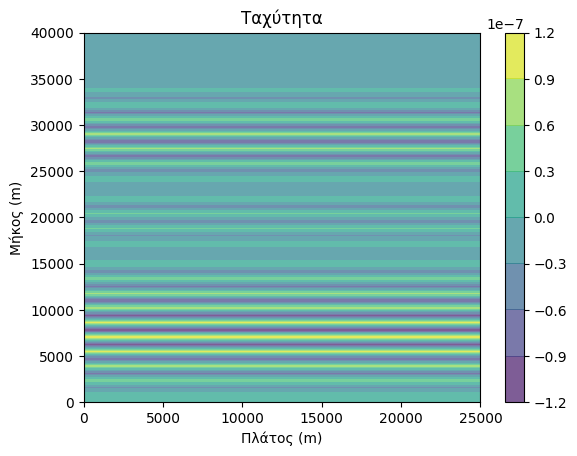
\includegraphics[scale=0.8]{1bcontour}}
	\caption{Αποτελέσματα \lat{1b}}
\end{figure}
\begin{figure}[h]
	\centering
	\subfigure[Διάγραμμα Ε.Ε. και ταχύτητας]{\label{fig:2aF}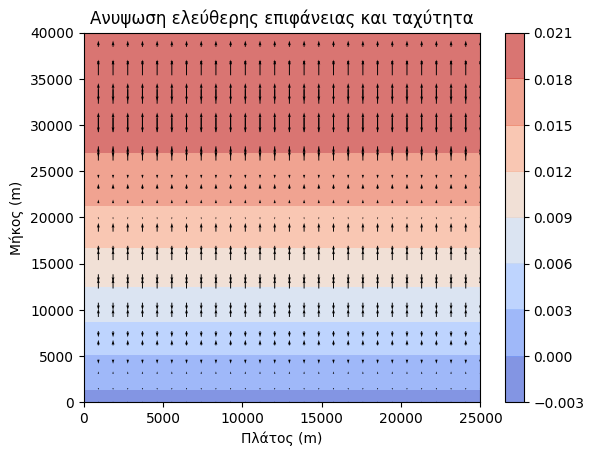
\includegraphics[scale=0.8]{2afinal_2d}}
	\subfigure[Διάγραμμα ταχύτητας σε κάτοψη]{\label{fig:2aV2d}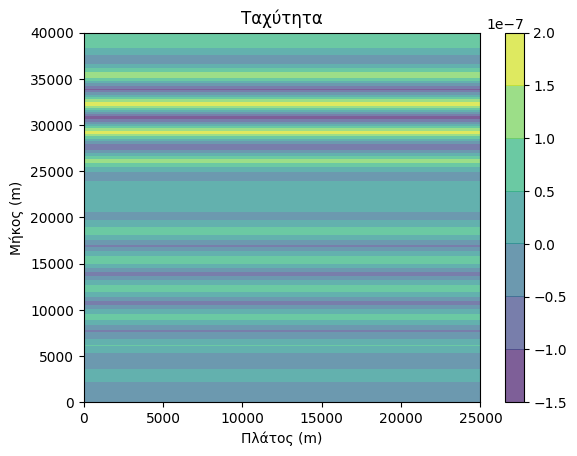
\includegraphics[scale=0.8]{2acontour}}
	\caption{Αποτελέσματα \lat{2a}}
\end{figure}
\begin{figure}[h]
	\centering
	\subfigure[Διάγραμμα Ε.Ε. και ταχύτητας]{\label{fig:2bF}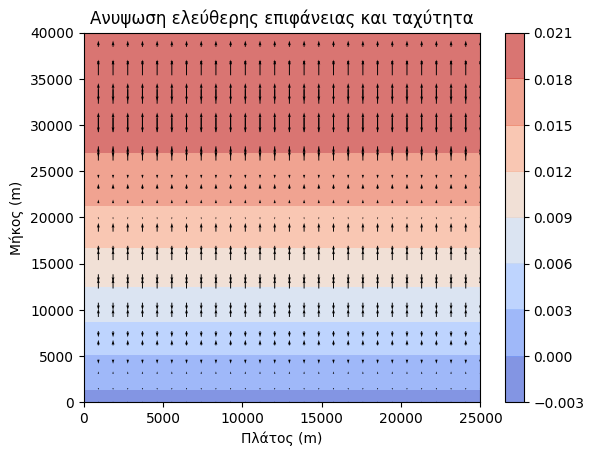
\includegraphics[scale=0.8]{2bfinal_2d}}
	\subfigure[Διάγραμμα ταχύτητας σε κάτοψη]{\label{fig:2bV2d}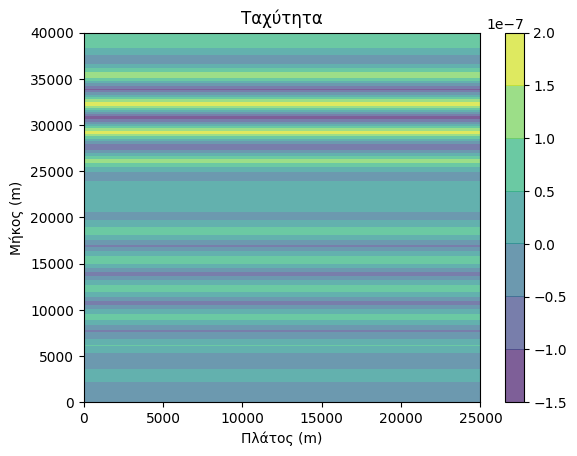
\includegraphics[scale=0.8]{2bcontour}}
	\caption{Αποτελέσματα \lat{2b}}
\end{figure}
\begin{figure}[h]
	\centering
	\subfigure[Διάγραμμα Ε.Ε. και ταχύτητας]{\label{fig:3aF}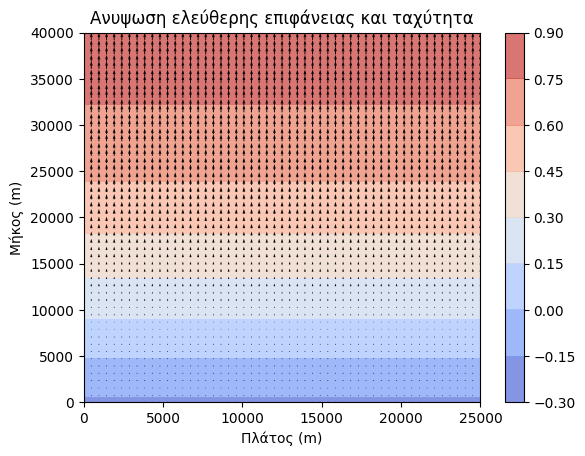
\includegraphics[scale=0.8]{3afinal_2d}}
	\subfigure[Διάγραμμα ταχύτητας σε κάτοψη]{\label{fig:3aV2d}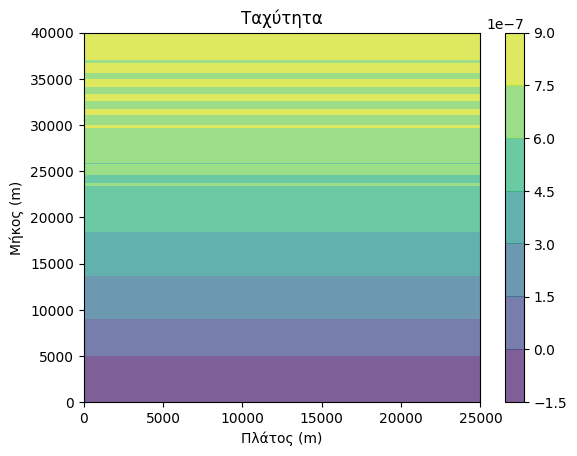
\includegraphics[scale=0.8]{3acontour}}
	\caption{Αποτελέσματα \lat{3a}}
\end{figure}
\begin{figure}[h]
	\centering
	\subfigure[Διάγραμμα Ε.Ε. και ταχύτητας]{\label{fig:3bF}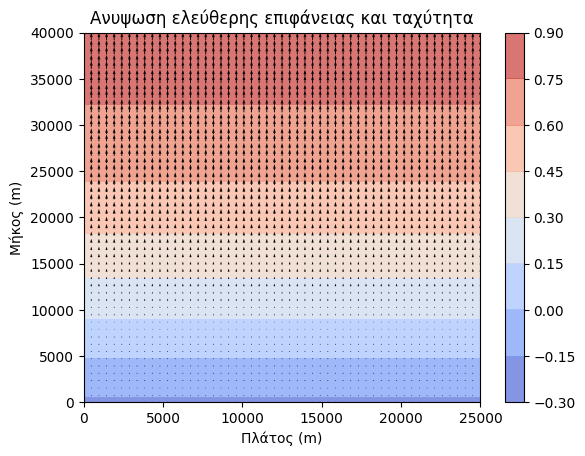
\includegraphics[scale=0.8]{3bfinal_2d}}
	\subfigure[Διάγραμμα ταχύτητας σε κάτοψη]{\label{fig:3bV2d}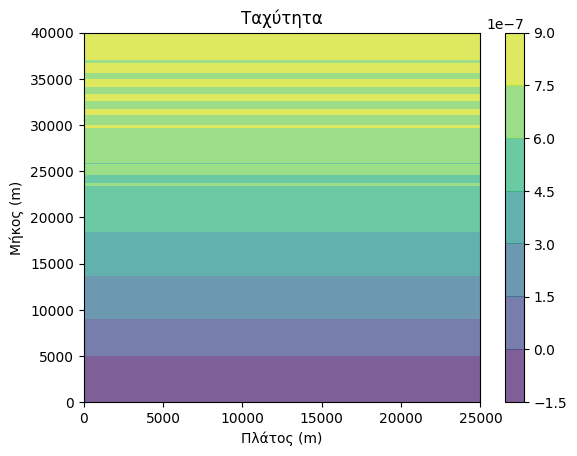
\includegraphics[scale=0.8]{3bcontour}}
	\caption{Αποτελέσματα \lat{3b}}
\end{figure}
\begin{figure}[h]
	\centering
	\subfigure[Διάγραμμα Ε.Ε. και ταχύτητας]{\label{fig:4aF}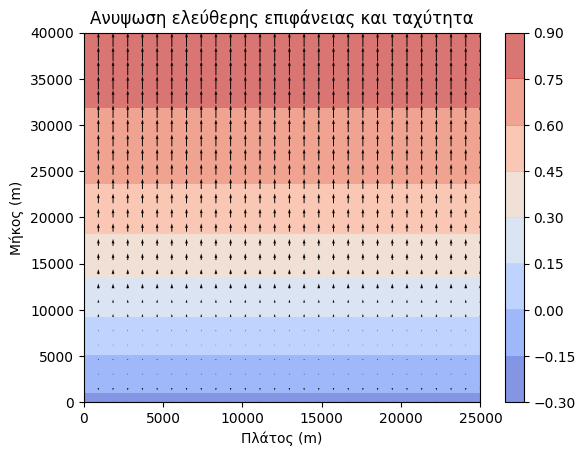
\includegraphics[scale=0.8]{4afinal_2d}}
	\subfigure[Διάγραμμα ταχύτητας σε κάτοψη]{\label{fig:4aV2d}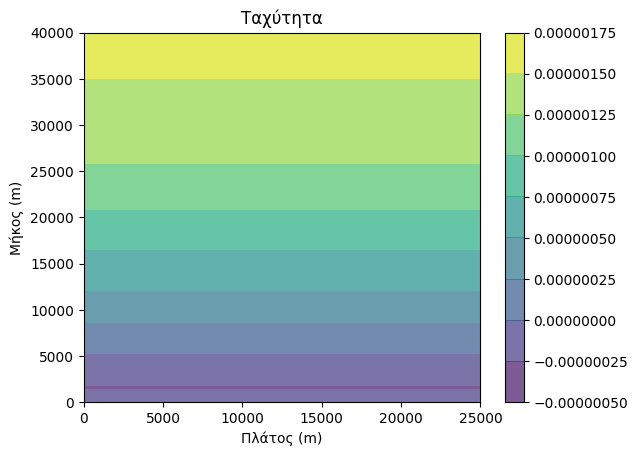
\includegraphics[scale=0.8]{4acontour}}
	\caption{Αποτελέσματα \lat{4a}}
\end{figure}
\begin{figure}[h]
	\centering
	\subfigure[Διάγραμμα Ε.Ε. και ταχύτητας]{\label{fig:4bF}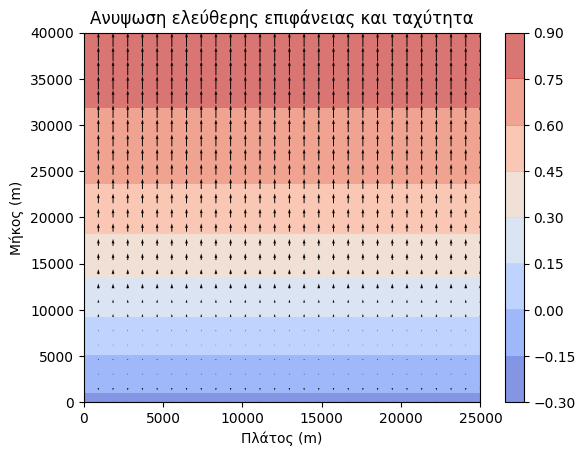
\includegraphics[scale=0.8]{4bfinal_2d}}
	\subfigure[Διάγραμμα ταχύτητας σε κάτοψη]{\label{fig:4bV2d}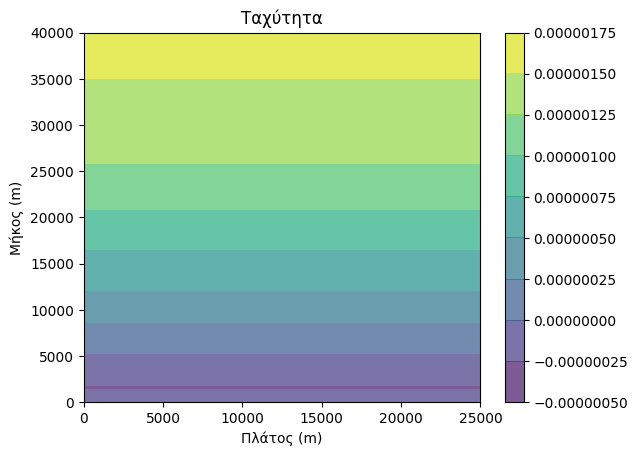
\includegraphics[scale=0.8]{4bcontour}}
	\caption{Αποτελέσματα \lat{4b}}
\end{figure}
\begin{figure}[h]
	\centering
	\subfigure[Διάγραμμα Ε.Ε. και ταχύτητας]{\label{fig:5aF}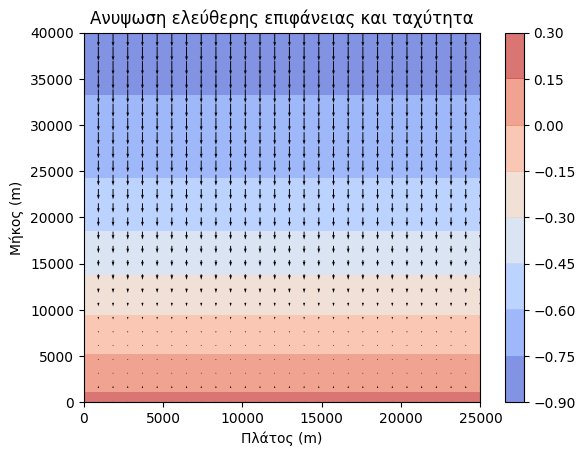
\includegraphics[scale=0.8]{5afinal_2d}}
	\subfigure[Διάγραμμα ταχύτητας σε κάτοψη]{\label{fig:5aV2d}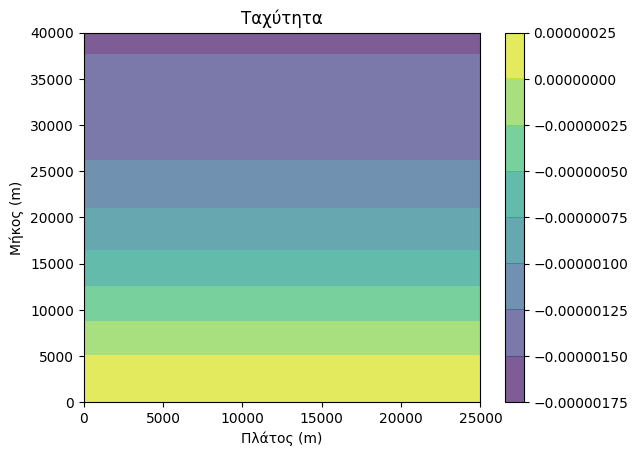
\includegraphics[scale=0.8]{5acontour}}
	\caption{Αποτελέσματα \lat{5a}}
\end{figure}
\begin{figure}[h]
	\centering
	\subfigure[Διάγραμμα Ε.Ε. και ταχύτητας]{\label{fig:5bF}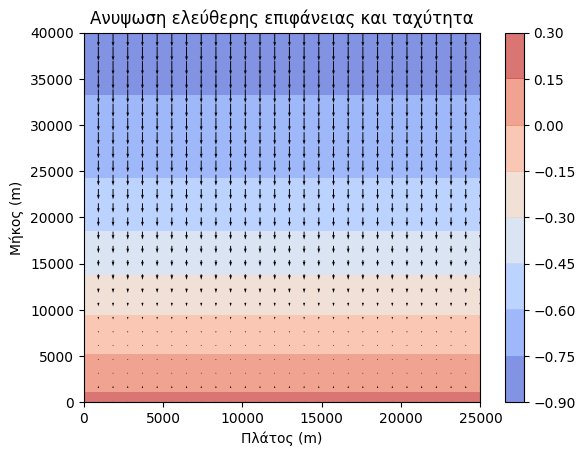
\includegraphics[scale=0.8]{5bfinal_2d}}
	\subfigure[Διάγραμμα ταχύτητας σε κάτοψη]{\label{fig:5bV2d}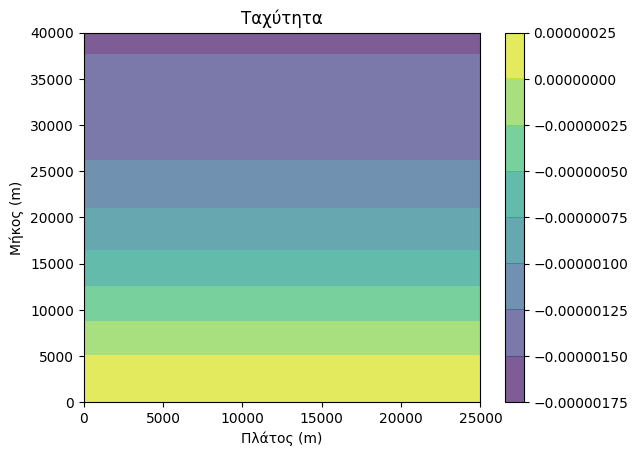
\includegraphics[scale=0.8]{5bcontour}}
	\caption{Αποτελέσματα \lat{5b}}
\end{figure}
\begin{figure}[h]
	\centering
	\subfigure[Χρονοσειρά ανύψωσης ελεύθερης επιφάνειας]{\label{fig:1a2aH}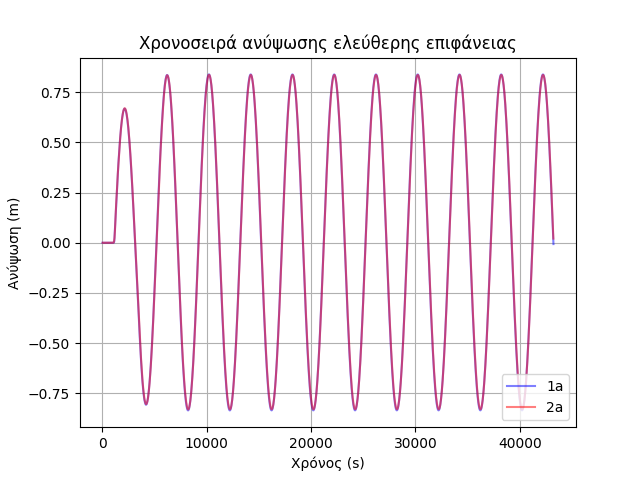
\includegraphics[scale=0.8]{1a2a-h}}
	\subfigure[Χρονοσειρά κατακόρυφης ταχύτητας]{\label{fig:1a2aV}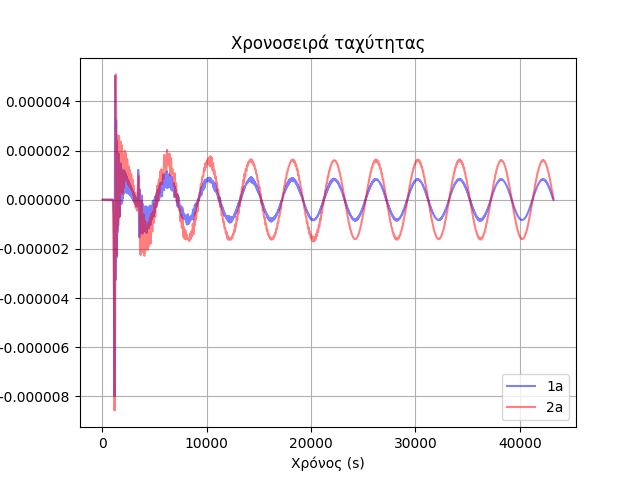
\includegraphics[scale=0.8]{1a2a-v}}
	\caption{Συγκριτικά αποτελέσματα χρονοσειρών 1a-2a}
\end{figure}
\begin{figure}[h]
	\centering
	\subfigure[Χρονοσειρά ανύψωσης ελεύθερης επιφάνειας]{\label{fig:1b2bH}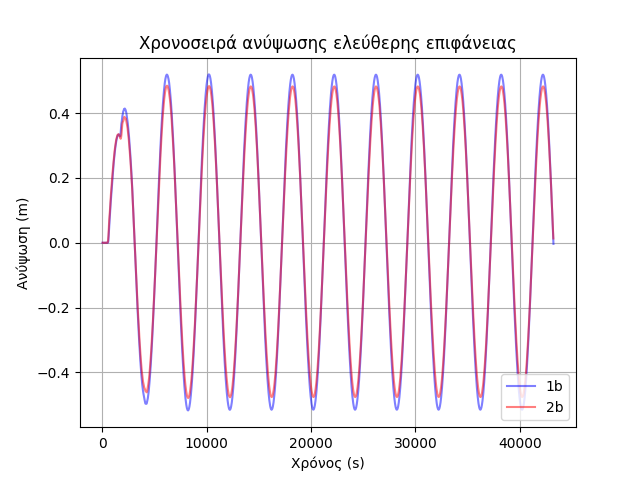
\includegraphics[scale=0.8]{1b2b-h}}
	\subfigure[Χρονοσειρά κατακόρυφης ταχύτητας]{\label{fig:1b2bV}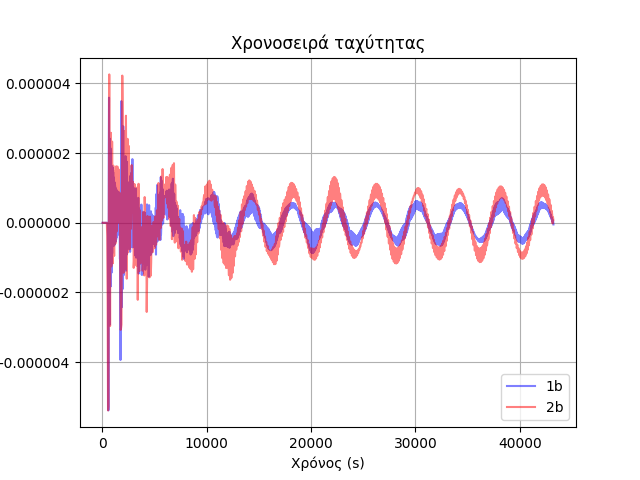
\includegraphics[scale=0.8]{1b2b-v}}
	\caption{Συγκριτικά αποτελέσματα χρονοσειρών 1b-2b}
\end{figure}
\begin{figure}[h]
	\centering
	\subfigure[Χρονοσειρά ανύψωσης ελεύθερης επιφάνειας]{\label{fig:3a4aH}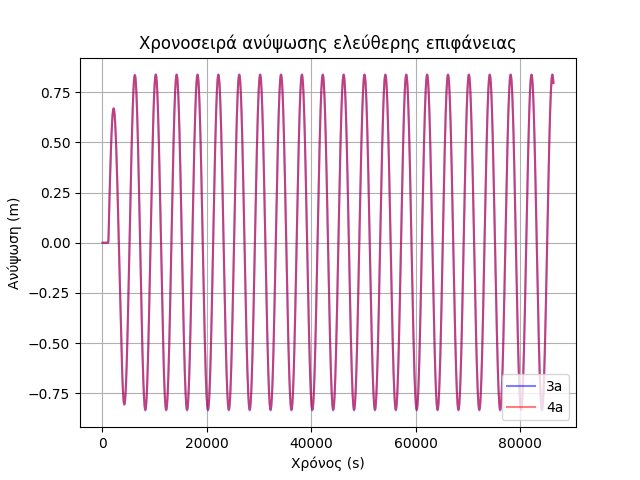
\includegraphics[scale=0.8]{3a4a-h}}
	\subfigure[Χρονοσειρά κατακόρυφης ταχύτητας]{\label{fig:3a4aV}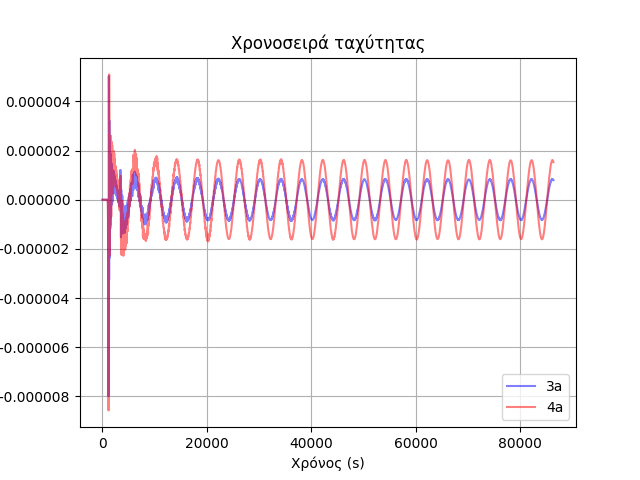
\includegraphics[scale=0.8]{3a4a-v}}
	\caption{Συγκριτικά αποτελέσματα χρονοσειρών 3a-4a}
\end{figure}
\begin{figure}[h]
	\centering
	\subfigure[Χρονοσειρά ανύψωσης ελεύθερης επιφάνειας]{\label{fig:3b4bH}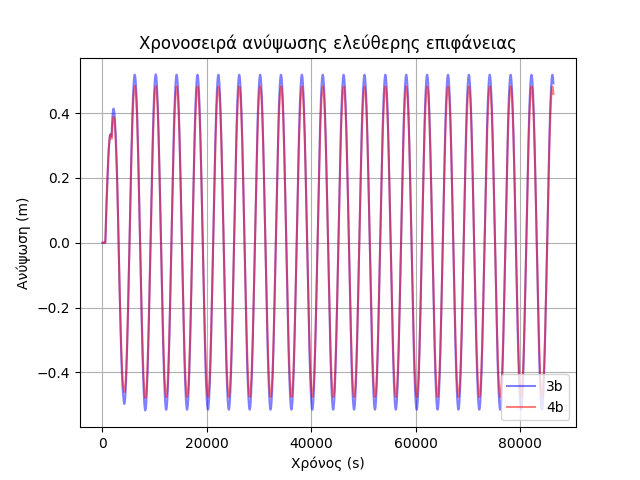
\includegraphics[scale=0.8]{3b4b-h}}
	\subfigure[Χρονοσειρά κατακόρυφης ταχύτητας]{\label{fig:3b4bV}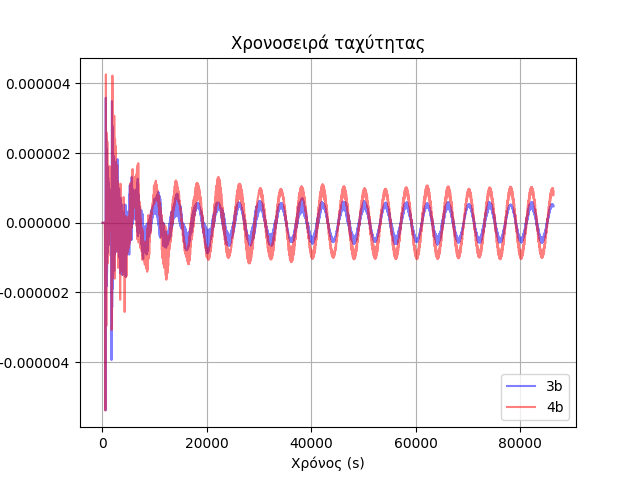
\includegraphics[scale=0.8]{3b4b-v}}
	\caption{Συγκριτικά αποτελέσματα χρονοσειρών 3b-4b}
\end{figure}

\cleardoublepage
\subsubsection{Σχολιασμός αποτελεσμάτων}
Τα αποτελέσματα από την παρουσίαση των διαγραμμάτων παρουσιάζουν ιδιαίτερο ενδιαφέρον. Όπως θα περίμενε κανείς όταν το πλέγμα γίνεται πιο πυκνό να υπάρχει μεγαύτερη ακρίβεια στον υπολογισμό των μεταβλητών του προβλήματος. Αντίθετα, φαίνεται, ότι κάτι τέτοιο δε συμβαίνει. Αυτό έγγυται στον περιορισμό \lat{CFL} που ανάλογα με το χωρικό βήμα αλλάζει αυτόματα και το χρονικό βήμα. Παρ' όλα αυτά, οι λύσεις συγκλίνουν και παρουσιάζουν συνοχή, ιδιαιτέρως σε μεγαλύτερους χρόνουν επίλυσης (1d, 5d).
Σε μεγάλους χρόνους επίλυσης, η ταχύτητα παρουσιάζει την αναμενόμενη συμπεριφορα, δηλαδή να κρατά σταθερό πρόσημο σε όλο το πλέγμα κάθε χρονική στιγμή, όπως φαίνεται από τα διαγράμματα \ref{fig:4aV2d}, \ref{fig:4bV2d}, \ref{fig:5aV2d} και \ref{fig:5bV2d}. 

Ενδιαφέρον παρουσιάζουν και τα διαγράμματα χρονοσειρών της ταχύτητας, καθώς παρατηρούμε το μεγάλο σφάλμα στον υπολογισμό για τις 2 πρώτες ώρες περίπου. Η λύση, όμως, ομαλοποιείται και λαμβάνει την αναμενόμενη ημιτονοειδή μορφή με το πέρασμα του χρόνου, όπου και σταθεροποιείται.

Όσον αφορά τα διαγράμματα χρονοσειράς της ανύψωσης της ελεύθερης επιφάνειας, παρατηρούμε ότι δημιουργείται στάσιμο κύμα πλάτους $2Α \approx 0.8m$, όπως φυσικά θα περίμενε κανείς, λόγω της πλήρους ανάκλασης.
	\cleardoublepage
	\nocite{*}
	\selectlanguage{greek}
	\lat{\bibliography{biblio}}

	\cleardoublepage



	\appendix
		\selectlanguage{english}
		\section{Αλγόριθμος επίλυσης του συστήματος \textlatin{Lorenz}}
		\pagestyle{appendix}
		\label{sec:lorenzPython}
		\lstset{style=withnums}
		\lstinputlisting[language=Python, caption=Αλγόριθμος επίλυσης του συστήματος \lat{Lorenz} σε \lat{Python}]{lorenz.py}
		\cleardoublepage
		\section{Υπολογισμός της τροχιάς υπό την επίδραση της δύναμης Coriolis σε \textlatin{Python}}
		\pagestyle{appendix}
		\label{sec:corPython}
		\lstset{style=withnums}
		\lstinputlisting[language=Python, caption=Τροχιά υπό την επίδραση της \lat{Coriolis} σε \lat{Python}]{coriolis.py}
		\cleardoublepage
		\section{Υπολογισμός ανύψωσης / ταπείνωσης ελεύθερης επιφάνειας}
		\pagestyle{appendix}
		\label{sec:waterLevelPython}
		\lstset{style=withnums}
		\lstinputlisting[language=Python, caption=Υπολογισμός ανύψωσης / ταπείνωσης ελεύθερης επιφάνειας]{waterLevel.py}
		\cleardoublepage
		\section{Υπολογισμός διανύσματος ταχύτητας}
		\pagestyle{appendix}
		\label{sec:velocityPython}
		\lstset{style=withnums}
		\lstinputlisting[language=Python, caption=Υπολογισμός διανύσματος ταχύτητας]{velocity.py}
 
\end{document}
